\documentclass[11pt]{article}

% Essential packages
\usepackage[margin=1in]{geometry}
\usepackage{amsmath,amssymb,amsthm}
\usepackage{mathtools}
\usepackage[numbers,square]{natbib}
\usepackage{booktabs}
\usepackage{hyperref}
\hypersetup{hypertexnames=false}
\usepackage{cleveref}
\usepackage{algorithm}
\usepackage{algpseudocode}
\usepackage{tikz}
\usetikzlibrary{decorations.pathreplacing}

% Theorem environments
\theoremstyle{definition}
\newtheorem{definition}{Definition}[section]

\theoremstyle{plain}
\newtheorem{theorem}{Theorem}[section]
\newtheorem{lemma}[theorem]{Lemma}
\newtheorem{corollary}[theorem]{Corollary}
\newtheorem{proposition}[theorem]{Proposition}

\theoremstyle{remark}
\newtheorem{remark}{Remark}[section]
\newtheorem{example}{Example}[section]

% Notation
\newcommand{\fhat}{\hat{f}}
\newcommand{\ghat}{\hat{g}}
\newcommand{\enc}{\mathrm{enc}}
\newcommand{\dec}{\mathrm{dec}}
\newcommand{\im}{\mathrm{Im}}
\newcommand{\TV}{d_{\mathrm{TV}}}
\newcommand{\B}{\{0,1\}}
% Cipher functor: \cipher{X} = C(X) when secret is implicit;
% \cipherS{X}{s} = C_s(X) when secret is explicit.
% Same notation applies to objects (latent types) and morphisms (latent functions):
% \cipherS{X}{s} = cipher value space; \cipherS{f}{s} = cipher map for f.
\newcommand{\cipher}[1]{\mathsf{C}(#1)}
\newcommand{\cipherS}[2]{\mathsf{C}_{#2}(#1)}
\DeclareMathOperator{\Uniform}{Uniform}

\title{Cipher Maps: Total Functions as Trapdoor Approximations}
\author{Alexander Towell\\\texttt{lex@metafunctor.com}}
\date{March 2026}

\begin{document}

\maketitle

\begin{abstract}
Outsourcing function evaluation to an untrusted machine typically
requires oblivious RAM (hiding access patterns), fully homomorphic
encryption (exact computation on ciphertexts), or garbled circuits
(encrypted lookup tables, single-use).  Each carries substantial cost.
We propose the \emph{cipher map}: a total function on bit strings whose
privacy properties emerge from a one-way trapdoor (a cryptographic
hash with a secret seed) combined with a frequency-equalized output
distribution.  Cipher maps fit the quantitative information flow
tradition~\cite{smith2009foundations,alvim2012measuring}: rather than
achieving negligible leakage in a security parameter, they bound
observable leakage by measurable parameters $\delta$ (representation
uniformity), $\varepsilon$ (noise-decode probability), and $\eta$
(correctness), with the entropy ratio serving as the security measure
(formal framework in companion work~\cite{towell2026maxconf}).  The
construction reduces to a single design choice: an \emph{acceptance
predicate} that partitions hash space among output values.  Acceptance
predicates expose a Pareto frontier between expected codeword length
$L$ and TV-leakage; the Shannon-optimal corner ($L = -\log_2
\varepsilon + H(Y)$, matching the information-theoretic lower bound)
and the TV-optimal corner are distinct under integer codeword
constraints, with the gap reaching $42\times$ in TV at $17\%$ length
overhead on heavy-tailed value distributions.  Composition is
predictable: the chain bound
$\eta_{\mathrm{total}} \leq 1 - \prod(1 - \eta_i)$ holds for sequential
composition, and a coincidence-oracle bound (accuracy $1 - \tfrac{1}{2}
\sum_y \alpha(y)^t$ for $t$ shared-$f$ instances under independent
seeds) characterizes multi-instance leakage and inverts the
single-instance Shannon recommendation at $t \geq 2$.  We formalize the
framework through four measurable properties, prove the
space-optimality, composition, and multi-instance theorems, validate
the Le Cam attacker bound empirically across a codec sweep, and
illustrate the construction on arbitrary maps, set membership, and
encrypted search.
\end{abstract}


%% ============================================================
\section{Introduction}
\label{sec:intro}

Consider a setting in which a trusted party wishes to outsource computation
to an untrusted machine.  The trusted party holds a function
$f : X \to Y$---a lookup table, a set membership predicate, an index---and
wants the untrusted machine to evaluate $f$ on encoded inputs without
learning $f$, $X$, or $Y$.

The central object of this paper is the \emph{cipher map}: a total function
$\fhat : \{0,1\}^n \to \{0,1\}^n$ that the untrusted machine evaluates
blindly.  The key insight is that $\fhat$ is total---every $n$-bit input
produces an $n$-bit output, with no concept of ``in-domain'' or
``out-of-domain.''  The notions of domain, correctness, false positive, and
false negative exist only on the trusted machine, which holds the encoding
and decoding functions (the trapdoor).  The untrusted machine sees only
opaque bit strings flowing through opaque total functions.

This paper develops the theory of cipher maps in a self-contained way.
We define four properties that characterize a cipher map
(\S\ref{sec:properties}), formalize the trusted/untrusted machine model
(\S\ref{sec:trust-model}), develop the batch construction unified under the
acceptance predicate framework (\S\ref{sec:batch}), prove the composition
theorem governing error accumulation (\S\ref{sec:composition}), and discuss
the online alternative via trapdoor Boolean algebra
(\S\ref{subsec:online}).

\paragraph{Contribution: framework, not new construction.}
We do not propose a new construction with novel space, time, or
correctness guarantees; rather, we identify a \emph{framework} (the
cipher map abstraction with four measurable properties and the
acceptance predicate apparatus) that unifies several existing
approximate-membership and frequency-hiding constructions under a
single formalism with measurable parameters $(\eta, \varepsilon, \delta,
\mu)$.  Bloom filters become cipher maps with $K(x) = 1$, exact
correctness ($\eta = 0$), and a degenerate acceptance partition;
prefix-free coding instantiates the entropy cipher map; Shannon-optimal
partition shaping unifies space optimality with frequency hiding
(\S\ref{subsec:acceptance}, \Cref{fig:acceptance-partition}).  The
contributions are the framework itself plus the formal results that
follow from it: an information-theoretic lower bound matched by the
construction (Theorems~\ref{thm:lower-bound}, \ref{thm:space-optimal}),
a composition theorem with error bounds
(Theorem~\ref{thm:composition}), a confidentiality bound tying
representation uniformity to a quantitative leakage measure
(Proposition~\ref{prop:confidentiality}), and a unification of three
prior threads (approximate data structures, frequency-hiding
encryption, encrypted search) under one abstraction.  Two further
contributions sharpen the value-side security analysis: a
multi-instance composition theorem
(Theorem~\ref{thm:coincidence-oracle}) characterizing equality-pattern
leakage when the same latent function is published as $t$ cipher maps
under independent seeds, and an empirical evaluation
(\S\ref{subsec:eval-codec-security}) confirming the Le Cam bound is
realized by the Bayes-optimal attacker across a sweep of acceptance
predicates and exposing a $42\times$ TV reduction available off the
single-instance Shannon-optimal corner.

\paragraph{Bernoulli error model.}
The error framework underlying cipher maps is the Bernoulli
model~\cite{bernoulli-types}.  Two axioms (element-wise independence and
conditional independence of block error rates) reduce the error model from
exponential complexity to two parameters per element.  This tractability is
what makes the composition theorem (Property~4) possible: errors combine
predictably because they are independent across elements.  The Bernoulli
model is developed independently; we reference it here only for the error
accounting that cipher maps inherit.

\paragraph{Positioning: parameterized leakage in the QIF tradition.}
Cipher maps belong to the \emph{quantitative information flow}
tradition~\cite{smith2009foundations,alvim2012measuring} and the broader
parameterized-leakage program initiated by entropic
security~\cite{dodis2005entropic}.  The defining commitment is that
security is \emph{measurable rather than negligible}: an untrusted
evaluator's residual uncertainty about the latent function is reported as
a continuous quantity (the \emph{entropy ratio} $e = H(Q)/n$ where $Q$
is the cipher value distribution observed by the untrusted evaluator
and $n$ is the cipher value space dimension), bounded below by the
cipher map's representation-uniformity parameter $\delta$ via the
Fannes--Audenaert continuity inequality (formal framework in companion
work~\cite{towell2026maxconf}).  This puts
cipher maps in a different design space from oblivious
RAM~\cite{goldreich1996software} (hides access patterns at polylog
overhead), fully homomorphic encryption~\cite{gentry2009fully} (preserves
exact algebraic structure on ciphertexts), and simulation-based
searchable encryption~\cite{curtmola2006searchable} (achieves
indistinguishability up to a leakage profile).  The closest structural
relative is the garbled circuit~\cite{yao1982protocols}, which also
encrypts a lookup table; cipher maps differ in being reusable,
approximate, and parameterized.  We make the contrast precise in
\S\ref{sec:related}.


%% ============================================================
\section{Related Work}
\label{sec:related}

Cipher maps draw on and differ from several lines of work in data
structures, cryptography, and secure computation.

\paragraph{Membership data structures.}
Bloom filters~\cite{bloom1970space} are the canonical approximate membership
structure: a bit array with $k$ hash functions, trading false positives for
space.  Quotient filters~\cite{bender2012quotient} and cuckoo
filters~\cite{fan2014cuckoo} improve cache locality and support deletion,
respectively, but share the same basic model.  Set membership (Remark~\ref{rem:membership}) subsumes Bloom filters as a special
case: a single hash function ($k=1$), exact correctness ($\eta=0$), and the
same information-theoretic space bound of $-\log_2\varepsilon$ bits per
element.  The difference is that the HashSet is a cipher map---a total
function on bit strings with a trapdoor---while Bloom filters expose their
output directly.

\paragraph{Perfect hash functions.}
Fredman, Koml\'{o}s, and Szemer\'{e}di~\cite{fredman1984storing} introduced
FKS perfect hashing with $O(n)$ space and $O(1)$ lookup.
Belazzougui, Botelho, and Dietzfelbinger~\cite{belazzougui2009hash} achieved
minimal perfect hash functions near the information-theoretic lower bound.
The batch cipher map construction (\S\ref{sec:batch}) is a perfect hash
function with a different optimization target: it maps domain elements to
prefix-free codewords (not to consecutive integers) and trades correctness
($\eta > 0$) for space, achieving $(1-\eta)(-\log_2\varepsilon + H(Y))$
bits per element.

\paragraph{Property-preserving encryption.}
Order-preserving encryption (OPE)~\cite{agrawal2004order,boldyreva2009order}
and deterministic encryption~\cite{bellare2007deterministic} enable
computation on ciphertexts by preserving algebraic structure (order,
equality).  Naveed et al.~\cite{naveed2015inference} demonstrated devastating inference
attacks exploiting exactly this preserved structure.  Cipher maps differ
fundamentally: rather than preserving structure at the cost of leakage,
cipher maps hide structure behind a total function.  The untrusted machine
cannot distinguish domain elements from noise, and the output distribution
is controlled by the representation uniformity parameter $\delta$.

\paragraph{Searchable symmetric encryption.}
Song, Wagner, and Perrig~\cite{song2000practical} introduced practical
encrypted keyword search.  Curtmola et al.~\cite{curtmola2006searchable}
formalized SSE with simulation-based security (IND-CKA).  Cash et
al.~\cite{cash2013highly} extended SSE to Boolean queries with sublinear
search.  SSE constructions use inverted indices and game-based security
definitions; cipher maps use total functions with information-theoretic
parameters ($\eta$, $\varepsilon$, $\delta$).  The approaches address
different threat models: SSE hides query results from the server (up to
leakage profiles), while cipher maps hide function identity and domain
membership through totality and noise closure.  The volume-hiding
line~\cite{kamara2019computationally} is closer to cipher maps' approach:
rather than analyzing leakage, it engineers indistinguishability between
document-set sizes.  Cipher maps achieve a related guarantee structurally
(totality plus Property~2) at lower per-query cost.

\paragraph{Frequency-hiding constructions.}
Kerschbaum's frequency-hiding OPE~\cite{kerschbaum2015frequency} hides
plaintext frequency by injecting random ranks on duplicate inserts;
cipher maps hide it by shaping the acceptance partition so that the
cipher value distribution matches the output distribution
(\S\ref{subsec:acceptance}, \Cref{fig:acceptance-partition}).  Both
attack the same threat (frequency analysis on encrypted records) by
different mechanisms: Kerschbaum randomizes duplicate ranks so that
frequency information cannot be recovered from rank ordering, while
cipher maps allocate hash-space partition widths $\alpha(y) \propto p_y$
so that frequency information cannot be recovered from output marginals.
The two constructions are complementary: Kerschbaum's mechanism applies
within each cipher map evaluation, the cipher map mechanism applies
across many evaluations.

\paragraph{Leakage-abuse attacks.}
A line of work demonstrates that the leakage permitted by SSE and PPE
security definitions is exploitable in practice.  Islam, Kuzu, and
Kantarcioglu~\cite{islam2012access} showed that access-pattern leakage on
SSE indices enables query recovery via background-knowledge attacks.
Naveed, Kamara, and Wright~\cite{naveed2015inference} demonstrated
devastating frequency- and inference-based attacks on PPE-encrypted
databases (OPE, deterministic encryption), recovering plaintext columns from
auxiliary data.  Cash, Grubbs, Perry, and
Ristenpart~\cite{cash2015leakage} showed that even SSE schemes with
leakage profiles formally analyzed under simulation-based definitions
remain vulnerable to query- and document-recovery attacks under realistic
adversary knowledge.
Cipher maps target the upstream causes of these attacks: rather than
permitting leakage and analyzing it, the four properties bound what
$U$ can observe.  Totality and Shannon-optimal acceptance allocation
together flatten the visible frequency profile (Property~2,
$\delta$-bounded), so frequency-based attacks face uniform output;
totality eliminates the ``in-domain vs.\ out-of-domain'' distinction
exploited by access-pattern attacks.  These structural defenses do not
make cipher maps immune to all leakage-abuse vectors: composition leaks
correlation structure (\S\ref{subsec:comp-leakage}), and a bounded query
budget combined with auxiliary data still gives the adversary statistical
advantage.

\paragraph{Honey encryption and ``every input decodes.''}
Honey encryption~\cite{juels2014honey} produces plausible-looking
plaintexts under any decryption key, defeating brute-force key search
because the adversary cannot tell a wrong key's output from a real
plaintext.  Cipher maps share the structural property that every input
produces output: there is no failure mode that signals ``wrong key'' or
``not in domain.''  But the targets differ.  Honey encryption protects
\emph{the encryption of a single message} against \emph{key recovery};
cipher maps protect \emph{the function $f$} against repeated function
evaluation by an untrusted evaluator.  Honey encryption is exact (a real
key recovers the real message); cipher maps are approximate (correctness
$1 - \eta$ even under the real trapdoor).  The shared intuition---that
ambiguity at decode time provides deniability---scales differently:
cipher maps' noise-decode probability $\varepsilon$ converts every cipher
output, including outputs under the real trapdoor, into a value that is
either the latent answer or a uniformly drawn alternative.

\paragraph{Garbled circuits and fully homomorphic encryption.}
Yao's garbled circuits~\cite{yao1982protocols} evaluate arbitrary functions
on encrypted inputs via encrypted lookup tables.  Gentry's fully homomorphic
encryption~\cite{gentry2009fully} enables exact computation on ciphertexts
without interaction.  Both achieve exact computation on encrypted data.
Cipher maps trade exactness for simplicity: a cipher map is a static lookup
table (one hash evaluation per query) with tunable error $\eta$, whereas
garbled circuits require per-gate encryption and are single-use, and FHE
incurs substantial computational overhead from noise management in lattice
operations.

\paragraph{Homophonic substitution.}
The representation uniformity property (multiple encodings per value,
$K(x) \propto 1/D(x)$) is a modern instance of homophonic
substitution~\cite{simmons1979symmetric}, in which frequent plaintext
symbols are assigned multiple ciphertext equivalents to flatten frequency
distributions.  The connection is direct: representation uniformity
generalizes homophonic substitution from substitution ciphers to arbitrary
total functions.


%% ============================================================
\section{The Cipher Map Abstraction}
\label{sec:abstraction}

\subsection{Preliminaries}

Throughout, $h : \{0,1\}^* \to \{0,1\}^n$ denotes a cryptographic hash
function modeled as a \emph{random oracle}~\cite{bellare1993random}: a
truly random function accessible to all parties via oracle queries.
Results stated ``under the random oracle model'' assume $h$ has this
property.  Elements of any finite type are encoded as bit strings before
hashing.

\paragraph{ROM dependence and standard-model considerations.}
All four properties and every theorem in this paper depend on the random
oracle model.  Practical instantiation uses cryptographic hash functions
(e.g., SHA-256, BLAKE3) whose pseudorandomness is conjectured but not
proven.  The critical ROM assumptions are:
\emph{(a)} uniform hash output on non-stored elements (Property~1,
totality, and the noise-decode probability $\varepsilon$);
\emph{(b)} independence of hash values across distinct elements
(Property~3, correctness analysis, and the construction-time bound of
Proposition~\ref{prop:construction-time});
\emph{(c)} independence across maps with distinct seeds
(Property~4, composition);
\emph{(d)} independence of hash values from the seed for unstored
inputs and across multiplicities $k \in \{0, \ldots, K(x)-1\}$
(Property~2, the $\delta$-bounded representation uniformity argument
underlying Proposition~\ref{prop:confidentiality}).
For domain-separated keyed hashes (HMAC-SHA256 with seed $\ell$ as the key),
each of these is widely accepted in practice.
A standard-model instantiation via universal hash families or pairwise-independent
constructions is an open question; we expect the four-property framework to
survive such a translation, but with explicit dependence on collision-resistance
and key-distinguishability assumptions.

\paragraph{Notational convention.}
We write $\cipherS{X}{s}$ for the cipher value space induced by encoding
the latent type $X$ under secret $s$, that is, the image of $\enc(\cdot,
\cdot)$ in $\B^n$.  When the secret is clear from context, we drop the
subscript and write $\cipher{X}$.  The same notation applies to latent
functions: for $f : X \to Y$, the cipher map of $f$ under secret $s$ is
written $\cipherS{f}{s} : \cipherS{X}{s} \to \cipherS{Y}{s}$.  Under the
random oracle model and the four properties developed in
\S\ref{sec:properties}, $\cipherS{\cdot}{s}$ behaves as a functor from
finite latent types to a category $\mathbf{Cipher}_s$ of cipher value
spaces: it takes objects (types) to objects and morphisms (functions) to
morphisms, and respects composition up to the error bound of
\S\ref{sec:composition} (exactly under the re-randomization condition,
Definition~\ref{def:re-randomization}).  The categorical apparatus,
including the rekeying functor $r_{s_1 \to s_2} :
\mathbf{Cipher}_{s_1} \to \mathbf{Cipher}_{s_2}$ and its information-theoretic
chain bound, is developed in companion work~\cite{towell2026rekeying};
in this paper we use the notation as a clarifying shorthand without
invoking the categorical machinery.

\subsection{Definition}

\begin{definition}[Cipher map]
\label{def:cipher-map}
Let $f : X \to Y$ be a \emph{latent function}.  A \emph{cipher map} for
$f$ is a tuple $(\fhat, \enc, \dec, s)$ where:
\begin{enumerate}
\item $\fhat : \{0,1\}^n \to \{0,1\}^n$ is a \textbf{total function} on
      $n$-bit strings;
\item $\enc : X \times \{0, \ldots, K(x){-}1\} \to \{0,1\}^n$ is an encoding
      function, where $K(x) \geq 1$ is the number of encodings for element $x$;
\item $\dec : \{0,1\}^n \to Y \cup \{\bot\}$ is a decoding function;
\item $s$ is a secret (the trapdoor) from which $\fhat$, $\enc$, and $\dec$
      are derived.
\end{enumerate}
The untrusted machine holds $\fhat$.  The trusted machine holds $\enc$,
$\dec$, and $s$.
\end{definition}

A cipher value $\enc(v, k)$ can be viewed as a cipher map for the constant
function $f_v(x) = v$: under this view, cipher values and cipher maps are
the same kind of object---a total function on bit strings---simplifying the
untrusted machine's interface.

\subsection{Two Construction Strategies}

Cipher maps arise from two fundamentally different construction strategies:

\begin{description}
\item[Batch construction.]  The trusted machine invests computation upfront
    to find a seed $s$ such that $\fhat$ satisfies correctness constraints
    for all $x \in X$ simultaneously.  This gives tunable correctness
    parameter $\eta$ and optimal space, but requires knowing $X$ and $f$ at
    construction time.  The entropy cipher map (\S\ref{sec:batch}) is the
    general batch construction.

\item[Online construction.]  The cipher map $\fhat$ is defined directly by
    the hash structure---no seed search is needed.  The secret $s$ is a hash
    key, not a searched seed.  Operations are limited to those the hash
    structure supports algebraically (e.g., set union, intersection).  Space
    and accuracy trade-offs are fixed by the hash width~$n$.  The trapdoor
    Boolean algebra (\S\ref{subsec:online}) is the online construction.
\end{description}

Both strategies produce objects satisfying Definition~\ref{def:cipher-map}.

\subsection{Construction Layers}
\label{subsec:layers}

The four properties (defined in \S\ref{sec:properties}) arise from three
orthogonal type transformations applied to the latent function.

\paragraph{Layer 1: Undefined injection.}
Extend the domain $X$ to $X \cup \{\bot_1, \ldots, \bot_N\}$ by adding $N$
undefined elements.  A function $f : X \to Y$ lifts to a partial function
$\tilde{f}$ that is undefined on the $\bot_i$.  Real elements become a
fraction $|X| / (|X| + N)$ of the extended type.  This controls the space
parameter $\varepsilon$ (the probability that random bits form a valid
codeword).

\paragraph{Layer 2: Noise closure.}
Lift the partial function $\tilde{f}$ to a total function $\fhat$ by
mapping undefined inputs to random outputs via cryptographic hash.  The
untrusted machine cannot distinguish real inputs from undefined
inputs---both produce $n$-bit output.  This yields \textbf{Property~1
(Totality)}.

\paragraph{Layer 3: Multiple representations.}
Replace each value $x$ with $K(x) \geq 1$ distinct representations, keyed
by the secret $s$.  Representational equality implies value equality, but
value equality does not imply representational equality.  Assigning
$K(x) \propto 1/D(x)$ equalizes frequencies.  This yields
\textbf{Property~2 (Representation Uniformity)}.

\medskip

The combined type is
$\mathrm{cipher}(\mathrm{noise}(\mathrm{undef}(X)))$---an element with
multiple representations, total evaluation, and diluted domain.
Properties~3 (Correctness) and~4 (Composability) are emergent: correctness
depends on the construction method; composability depends on the totality
guarantee enabling chained evaluation.

These layers are conceptual scaffolding explaining \emph{why} each property
exists, not algebraic monads.  Whether the layers satisfy formal monad
laws in the approximate setting is an open question (see \S\ref{sec:discussion}).


%% ============================================================
\section{Four Properties}
\label{sec:properties}

A cipher map $(\fhat, \enc, \dec, s)$ for $f : X \to Y$ is characterized by
four properties parameterized by $(\eta, \varepsilon, \mu, \delta)$
(summarized in Table~\ref{tab:params}).

\subsection{Property 1: Totality}

\begin{definition}[Totality]
\label{def:totality}
The function $\fhat : \{0,1\}^n \to \{0,1\}^n$ is \emph{total}: for every
$c \in \{0,1\}^n$, $\fhat(c) \in \{0,1\}^n$.  For $c$ chosen uniformly at
random from $\{0,1\}^n \setminus \im(\enc)$, the distribution of $\fhat(c)$
is uniform over $\{0,1\}^n$ under the random oracle model.
\end{definition}

Totality ensures that the untrusted machine cannot distinguish a real query
$\enc(x, k)$ from a random filler string $c \gets \{0,1\}^n$, because both
produce $n$-bit outputs.  If out-of-domain queries returned an error or
$\bot$, the untrusted machine could identify real queries by observing which
inputs produce valid output.

\subsection{Property 2: Representation Uniformity (\texorpdfstring{$\delta$}{delta}-bounded)}

\begin{definition}[Representation uniformity]
\label{def:rep-uniformity}
Let $D$ be a distribution on $X$.  Define the induced distribution on cipher
values:
\begin{equation}
Q(c) = \sum_{x \in X} D(x) \cdot \frac{|\{k : \enc(x,k) = c\}|}{K(x)}.
\end{equation}
The cipher map has \emph{$\delta$-representation uniformity} if
\begin{equation}
\TV(Q,\, \Uniform(\{0,1\}^n)) \leq \delta,
\end{equation}
where $\TV$ is total variation distance.
\end{definition}

Total variation distance has the operational interpretation that no
statistical test can distinguish $Q$ from uniform with advantage exceeding
$\delta$.  To achieve small $\delta$, assign $K(x) \propto 1/D(x)$
encodings per value (homophonic substitution), so that frequent values get
more representations.

\begin{remark}[Marginal uniformity only]
\label{rem:marginal-only}
Representation uniformity bounds the \emph{marginal} distribution of
individual cipher values.  It says nothing about \emph{joint} distributions:
an adversary observing sequences of cipher values can still detect
correlations.  See \S\ref{subsec:granularity} for the encoding granularity
trade-off.
\end{remark}

\subsection{Property 3: Correctness (\texorpdfstring{$\eta$}{eta}-bounded)}

\begin{definition}[Correctness]
\label{def:correctness}
For $x$ chosen uniformly from $X$ and $k$ chosen uniformly from
$\{0, \ldots, K(x)-1\}$:
\begin{equation}
\Pr_{x,k}\bigl[\dec(\fhat(\enc(x,k))) \neq f(x)\bigr] \leq \eta.
\end{equation}
\end{definition}

The parameter $\eta \in [0,1)$ is a \emph{construction} parameter: it
reflects how many constraints the seed $s$ must satisfy.  Tolerating
$\eta > 0$ makes the seed search faster and the structure smaller.  Once
built, the failing elements are deterministic for a given seed---the same
elements always fail.

\begin{remark}[Approximation as privacy]
Nonzero $\eta$ also provides privacy: a false positive creates plausible
deniability, since the untrusted machine cannot distinguish ``element is in
the set'' from ``cipher map erred.''  With $\eta = 0$, the answer is
deterministic; with $\eta > 0$, each answer carries ambiguity.
\end{remark}

\subsection{Property 4: Composability}

\begin{definition}[Composability]
\label{def:composability}
The composition of two cipher maps is again a cipher map.  Specifically,
let $\cipherS{f}{s} : \cipherS{X}{s} \to \cipherS{Y}{s}$ be a cipher map
for $f : X \to Y$ and $\cipherS{g}{s} : \cipherS{Y}{s} \to \cipherS{Z}{s}$
a cipher map for $g : Y \to Z$ (both under the same secret~$s$, sharing
encoding and decoding for type $Y$).  Then
\[
\cipherS{g}{s} \circ \cipherS{f}{s} \;:\; \cipherS{X}{s} \to \cipherS{Z}{s},
\]
defined by $(\cipherS{g}{s} \circ \cipherS{f}{s})(c) = \cipherS{g}{s}(\cipherS{f}{s}(c))$,
realizes a cipher map for $g \circ f : X \to Z$.  In tuple form: if
$(\fhat, \enc_f, \dec_f, s)$ and $(\ghat, \enc_g, \dec_g, s)$ are the
underlying cipher maps for $f$ and $g$, the composition has cipher
function $\ghat \circ \fhat$, encoding $\enc_f$, and decoding $\dec_g$.
\end{definition}

\begin{remark}[Master secret vs.\ operational sub-derivations]
\label{rem:master-vs-op}
Throughout this paper, ``under secret $s$'' refers to the master secret
shared across the cipher map family.  Each individual cipher map's
hash randomization derives from $s$ via a domain separator unique to
the cipher map (e.g., the operational seed for $\cipherS{f}{s}$ is
$\mathit{op\_seed}_f = \mathrm{HMAC}(s, \texttt{"f"})$).  Under the
random oracle model, distinct cipher maps under the same master secret
have independent operational seeds; this independence is what makes the
re-randomization condition (Definition~\ref{def:re-randomization}) the
typical case rather than an exception.
\end{remark}

Composability is enabled by totality: since $\cipherS{f}{s}$ is total,
its output is always a valid $n$-bit input to $\cipherS{g}{s}$.  The
untrusted machine can chain cipher maps without needing to decode
intermediate results.  In functorial language, $\cipherS{\cdot}{s}$
takes the latent composition $g \circ f$ to the cipher composition
$\cipherS{g}{s} \circ \cipherS{f}{s}$, agreeing exactly under the
re-randomization condition (Definition~\ref{def:re-randomization}) and
up to the bound of Theorem~\ref{thm:composition} otherwise.  Composing
across different secrets requires the rekeying functor of
\cite{towell2026rekeying}; we restrict attention to single-secret
composition in this paper.

\begin{theorem}[Composition correctness]
\label{thm:composition-correctness}
Under the hypotheses of Definition~\ref{def:composability}, if $\fhat$ has
correctness $\eta_f$ and $\ghat$ has correctness $\eta_g$, then
$\ghat \circ \fhat$ has correctness
\[
\eta_{g \circ f} \leq \eta_f + \eta_g - \eta_f \eta_g
  = 1 - (1 - \eta_f)(1 - \eta_g),
\]
with equality under the re-randomization condition (see
\S\ref{sec:composition}, Theorem~\ref{thm:composition} and
Definition~\ref{def:re-randomization}).
\end{theorem}

\begin{remark}[Noise under composition]
Noise input to $\fhat$ produces random output (by totality).  With
probability $\varepsilon$, that random output happens to be a valid codeword
for $\ghat$.  We do not try to control noise output---the cipher map is just
a hash.  This is a feature: valid-looking outputs do not prove valid inputs.
\end{remark}

\subsection{Parameter Decomposition}

\begin{table}[ht]
\centering
\caption{Cipher map parameters.}
\label{tab:params}
\begin{tabular}{@{}llll@{}}
\toprule
Parameter & Range & Controls & Determined by \\
\midrule
$\eta$ (correctness) & $[0,1)$ & Fraction of wrong answers &
    Construction (seed search) \\
$\varepsilon$ (noise decode) & $(0,1)$ & Pr[random bits valid] &
    Encoding scheme \\
$\mu$ (value cost) & $(0,\infty)$ & Bits per element for values &
    $\mu = H(Y)$ \\
$\delta$ (uniformity) & $[0,1]$ & TV distance from uniform &
    Multiplicity $K(x)$ \\
$K(x)$ (multiplicity) & $\{1,2,\ldots\}$ & Encodings per element &
    Set to $\propto 1/D(x)$ \\
$p$ (entanglement) & $\{1, \ldots, k\}$ & Encoding granularity &
    Correlation structure (\S\ref{subsec:granularity}) \\
\bottomrule
\end{tabular}
\end{table}

The space per element decomposes as:
\[
\text{bits/element} = -\log_2 \varepsilon + \mu = -\log_2 \varepsilon + H(Y),
\]
where $-\log_2 \varepsilon$ bits distinguish signal from noise and $H(Y)$
bits encode the function value.  This decomposition is
information-theoretic.


%% ============================================================
\section{The Trusted/Untrusted Machine Model}
\label{sec:trust-model}

The four properties take operational meaning through a two-party model.
Throughout, we adopt the standard adversary convention from quantitative
information flow~\cite{smith2009foundations}: the untrusted machine~$U$
is \emph{honest-but-curious}, faithfully evaluating $\fhat$ on every
input it receives but attempting to learn information about the latent
function $f$, the domain $X$, the codomain $Y$, or specific values from
the observed input/output trace.  Active deviations (returning incorrect
results, refusing queries, inserting its own queries) are out of scope
for this paper; they are addressable by orthogonal verification or
auditing layers, but the parameterized leakage we analyze is the same.

\begin{definition}[Trusted machine $T$]
\label{def:trusted}
The trusted machine $T$ holds: the seed $s$ (trapdoor), the encoding
function $\enc$, the decoding function $\dec$, and knowledge of which
queries are real vs.\ filler.

$T$ can:
\begin{enumerate}
\item Encode plaintext values: $x \mapsto \enc(x, k)$ for chosen $k$.
\item Decode cipher results: $r \mapsto \dec(r)$.
\item Inject noise: generate random $c \gets \{0,1\}^n$ as filler queries.
\item Verify results: check $\dec(\fhat(\enc(x,k))) = f(x)$.
\item Reseed: construct a new cipher map with fresh $s'$ when leakage accumulates.
\end{enumerate}
\end{definition}

\begin{definition}[Untrusted machine $U$]
\label{def:untrusted}
The untrusted machine $U$ holds: the cipher map $\fhat$ (a total function
on bit strings) and a collection of cipher values (encodings plus filler,
indistinguishable to $U$).

$U$ can:
\begin{enumerate}
\item Evaluate cipher maps: $c \mapsto \fhat(c)$ for any
    $c \in \{0,1\}^n$.
\item Return results to $T$.
\item Compute arbitrary functions of its observed
    trace $\tau = ((c_i, \fhat(c_i)))_{i \in [N]}$.
\end{enumerate}

$U$'s view of the latent function $f$ is the trace $\tau$ together with
the cipher map $\fhat$.  We analyze what $U$ can learn from this view as
a quantitative leakage measure rather than as a binary security event.
\end{definition}

\subsection{The Confidentiality Measure}
\label{subsec:conf-measure}

We adopt the \emph{entropy ratio} of the companion entropy ratio
paper~\cite[\S 4]{towell2026maxconf}.

\begin{definition}[Entropy ratio]
\label{def:entropy-ratio}
Let $Q$ denote the distribution of cipher values that $U$ observes
(the marginal of the trace's input column).  The \emph{entropy ratio}
of $U$'s view is
\[
e(\fhat, \tau) \;=\; H(Q) \,/\, n,
\]
where $H(Q)$ is the Shannon entropy of $Q$ and $n$ is the cipher value
space dimension (so the maximum-entropy reference is the uniform
distribution on $\B^n$, with entropy $n$ bits).  The entropy ratio
satisfies $0 \leq e \leq 1$: $e = 1$ corresponds to a uniformly
distributed cipher value stream (no marginal leakage from the cipher
value distribution alone), and $e \to 0$ corresponds to a degenerate
stream concentrated on few values.
\end{definition}

This normalized form of Shannon leakage is standard in the quantitative
information flow tradition~\cite{smith2009foundations,alvim2012measuring}
and the entropic security literature~\cite{dodis2005entropic}.  We use
Shannon entropy rather than min-entropy because the relevant adversary
goal in this paper is \emph{average-case} information recovery from
many cipher value observations (where Shannon entropy gives the
information-theoretic ceiling on the adversary's expected gain),
not single-try guessing (where min-entropy is more natural).  Settings
where min-entropy is preferred (one-shot key recovery, cryptographic
guessing games) are treated in the companion
work~\cite[\S 4]{towell2026maxconf}.

We record only the bridge to the cipher map parameters here; formal
definitions, decomposition into multiple components, and discussion of
when this measure suffices versus when other QIF measures (min-entropy
leakage, $g$-leakage) apply, all appear
in~\cite[\S 4]{towell2026maxconf}.

\begin{proposition}[Confidentiality bound for cipher maps]
\label{prop:confidentiality}
Let $(\fhat, \enc, \dec, s)$ be a cipher map with
representation-uniformity parameter $\delta \leq 1/2$ over an $n$-bit
cipher value space (Property~2).  Then the entropy ratio of $U$'s view
satisfies
\begin{equation}
\label{eq:fannes-bridge}
e(\fhat, \tau) \;\geq\; 1 - \delta - h_2(\delta) / n,
\end{equation}
where $h_2(\delta) = -\delta \log_2 \delta - (1 - \delta) \log_2(1 - \delta)$
is the binary entropy.  The condition $\delta \leq 1/2$ is the standard
applicability range of the Fannes--Audenaert continuity inequality; for
$\delta > 1/2$ the bound is trivial ($e \geq 0$).
\end{proposition}

\begin{proof}[Proof sketch]
Property~2 gives $\TV(Q, \mathrm{Uniform}) \leq \delta$ where $Q$ is the
cipher value distribution induced by $\enc$ on the $\B^n$ ambient space.
Applying the Fannes--Audenaert continuity inequality with reference
distribution $\mathrm{Uniform}(\B^n)$ (entropy $n$) gives
$H(Q) \geq n(1 - \delta) - h_2(\delta)$, and dividing by $n$ yields
\eqref{eq:fannes-bridge}.  Full proof and discussion of tightness in
\cite[Theorem~4.1, part~3]{towell2026maxconf}.  The bound applies
specifically to the cipher value marginal; downstream bounds on what
$U$ can learn about the latent function $f$ or the latent input $X$
follow by data-processing arguments
(\S\ref{subsec:operational}).
\end{proof}

\begin{remark}[The role of $\delta$]
\label{rem:delta-role}
Proposition~\ref{prop:confidentiality} reduces confidentiality engineering
for cipher maps to the concrete problem of minimizing $\delta$.  Three
mechanisms reduce $\delta$, each with explicit costs analyzed in the
companion work: noise injection (bandwidth cost), multiple representations
$K(x) > 1$ (storage cost; Simmons homophonic prescription), and joint
encoding granularity (storage cost growing as $|Y|^k$).  We discuss the
multiplicity mechanism in \S\ref{subsec:granularity}; the others are out
of scope for this paper.
\end{remark}

\subsection{Operational Consequences}
\label{subsec:operational}

From the bound \eqref{eq:fannes-bridge} together with the four properties,
several operational consequences follow that may be more familiar to
readers expecting binary security claims.  These are not separate
security guarantees; they are concrete restatements of the entropy ratio
bound under specific adversary goals.

\begin{enumerate}
\item \emph{Decoding requires the trapdoor.}  Recovering $\dec$ from
    $\fhat$ requires inverting the cryptographic hash $h$ used in the
    construction (\S\ref{sec:batch}).  Under the random oracle model
    (Preliminaries, \S\ref{sec:abstraction}), this is computationally
    infeasible.
\item \emph{Real and filler queries are $\delta$-equivocal in
    distribution (Properties~1 and 2 together).}  Both are observed as
    $n$-bit cipher values, and the cipher value distribution is
    $\delta$-close to uniform by Property~2.  Consequently, no
    statistical test distinguishes real from filler with advantage
    exceeding $\delta/2$ (Le Cam's two-point
    lemma~\cite{lecam1986asymptotic} applied to the cipher value
    marginals; we report $\delta$ as a conservative upper bound
    throughout to match the total-variation normalization).  The same
    Le Cam bound applies at the decoded-value level
    (\S\ref{subsec:eval-codec-security}), where it limits any
    membership-inference attacker observing $\dec(\fhat(c))$ to
    accuracy $1/2 + \delta/2$ at balanced class prior.
\item \emph{Domain identification is bounded by~$\delta$ (Property~2).}
    For any binary discrimination question $U$ poses (e.g., ``is this
    cipher value a real domain element or noise?''), $U$'s advantage
    over random guessing is at most $\delta$, by the data-processing
    inequality applied to Property~2's TV bound.  Aggregated over $N$
    independent observations, $U$'s advantage on a recovery game grows
    no faster than the entropy ratio bound of
    Proposition~\ref{prop:confidentiality} permits.
\item \emph{Function-value leakage is bounded by the entropy ratio.}
    For any function $g(f)$ that $U$ wishes to extract, $U$'s
    information gain (mutual information between the trace and
    $g(f)$) is bounded above by $n(1 - e(\fhat, \tau))$ bits, by the
    data-processing inequality applied to
    Proposition~\ref{prop:confidentiality}.  Translating this bit
    bound into a guessing-advantage bound depends on the prior over
    $g(f)$ and is treated for specific adversary games
    in~\cite[\S 5--6]{towell2026maxconf}.
\end{enumerate}

\paragraph{Protocol.}
The information flow is:
\begin{enumerate}
\item $T$ encodes inputs: $\enc(x_1, k_1), \ldots, \enc(x_m, k_m)$.
\item $T$ generates filler: $c_1, \ldots, c_r \gets \{0,1\}^n$.
\item $T$ sends all cipher values (real plus filler, shuffled) to $U$.
\item $U$ evaluates $\fhat$ on each cipher value and returns results.
\item $T$ decodes the results it cares about and discards filler results.
\end{enumerate}

\begin{table}[ht]
\centering
\caption{Quantitative confidentiality bounds against $U$ (honest-but-curious).
The entropy ratio $e$ is the unifying measure;
Proposition~\ref{prop:confidentiality} ties it to $\delta$ via the
Fannes--Audenaert continuity inequality.}
\label{tab:guarantees}
\begin{tabular}{@{}lll@{}}
\toprule
Adversary goal & Bound & Mechanism \\
\midrule
Distinguish real from filler & $\TV \leq \delta$ & Totality + Property~2 \\
Frequency-analyze cipher values & $\TV \leq \delta$ & Property~2 (uniformity) \\
Recover plaintext value $f(x)$ & $1 - e$ advantage & Prop.~\ref{prop:confidentiality} via $\delta$ \\
Test membership $x \in X$ & $\delta$-bounded & Totality + Property~2 \\
Detect cross-query correlations & \textbf{Not bounded} & Marginal uniformity only (\S\ref{subsec:comp-leakage}) \\
\bottomrule
\end{tabular}
\end{table}

The last row is the honest limitation: marginal $\delta$-uniformity per
cipher map does not bound joint correlations across multiple cipher maps
sharing inputs.  The compositional leakage analysis in
\S\ref{subsec:comp-leakage} treats this case; the encoding granularity
parameter $p$ controls the trade-off between space and joint correlation
hiding.


%% ============================================================
\section{The Batch Construction}
\label{sec:batch}

The batch construction requires knowing $X$ and $f$ at construction time
and invests computation in a seed search to find a cipher map satisfying
correctness constraints for all stored elements.  This section develops the
batch construction from the information-theoretic lower bound through the
acceptance predicate framework, culminating in the entropy cipher map---the
general batch cipher map for arbitrary $f : X \to Y$.

\subsection{Information-Theoretic Lower Bound}
\label{subsec:lower-bound}

\begin{theorem}[Lower bound]
\label{thm:lower-bound}
Any data structure representing an approximate map $\fhat$ for
$f : X \to Y$ with noise decode probability $\varepsilon$ and correctness
$\eta = 0$ over $n$ stored elements requires at least
\begin{equation}
n\bigl(-\log_2 \varepsilon + H(Y)\bigr) \text{ bits},
\end{equation}
or equivalently $-\log_2 \varepsilon + H(Y)$ bits per element.
\end{theorem}

\begin{proof}
The bound decomposes into two independent information requirements.

\emph{Membership component.}
Consider the membership predicate $\dec(\fhat(c)) \neq \bot$.  For a
universe $U$ with $|U| \gg n$, the structure must distinguish $n$ stored
elements from $|U|-n$ non-elements, with at most an $\varepsilon$ fraction
of non-elements decoding to valid output.  There are $\binom{|U|}{n}$
possible sets of size $n$ from a universe $U$.  Any representation must
distinguish all such sets, requiring at least $\log_2 \binom{|U|}{n}$
bits.  For $|U| \gg n$, Stirling's approximation
$\log_2 \binom{|U|}{n} = n \log_2(|U|/n) + n \log_2 e + O(\log n)$ gives
$\log_2 \binom{|U|}{n} \approx n \log_2(|U|/n)$ bits to leading order in
$|U|/n$, or $\log_2(|U|/n)$ bits per element.  We drop the $n \log_2 e
\approx 1.44 n$ subleading term: it is independent of $|U|$ and adds at
most a constant overhead per element, which the matching achievability
construction (Theorem~\ref{thm:space-optimal}) matches asymptotically.  The noise-decode probability
$\varepsilon$ is the fraction of bit strings in $\{0,1\}^n$ that decode to
some valid output value: under any membership-faithful encoding, exactly
the $n$ stored elements decode validly out of the $|U|$ universe inputs,
so $\varepsilon = n / |U|$ when the universe is identified with the
$n$-bit cipher value space.  Substituting yields
$n \log_2(1/\varepsilon)$ bits.

\emph{Value component.}
Independently of membership, the structure must encode the function values
$(f(x_1), \ldots, f(x_n))$.  By Shannon's source coding theorem~\cite{shannon1948mathematical}, encoding
$n$ independent draws from the distribution $(p_y)$ requires at least
$n H(Y)$ bits.

Since membership and value encoding are jointly necessary, the total
requirement is $n(-\log_2 \varepsilon + H(Y))$ bits.  The additivity holds
because the membership bits and value-encoding bits convey independent
information: by the entropy chain rule,
$H(\text{membership}, \text{value}) = H(\text{membership}) + H(\text{value} \mid \text{membership})$,
and conditioning on membership (i.e., knowing which elements are stored) does
not reduce the entropy of the value assignment, since the values
$(f(x_1), \ldots, f(x_n))$ are an independent degree of freedom.
\end{proof}

\subsection{Acceptance Predicates}
\label{subsec:acceptance}

The construction depends on a rule for deciding whether a hash value
encodes a particular output.  We abstract this as an \emph{acceptance
predicate}.

\begin{definition}[Acceptance predicate]
\label{def:acceptance}
An acceptance predicate for codomain $Y$ is a family of disjoint sets
$\{A(y) \subseteq \{0,1\}^n : y \in Y\}$.  The decoder is
$\dec(\text{hash}) = y$ if $\text{hash} \in A(y)$, and $\bot$ otherwise.
The acceptance probability for value $y$ is $\alpha(y) = |A(y)| / 2^n$,
and the noise-decode probability is
$\varepsilon = \sum_y \alpha(y) = |\bigcup_y A(y)| / 2^n$.
\end{definition}

\begin{figure}[ht]
\centering
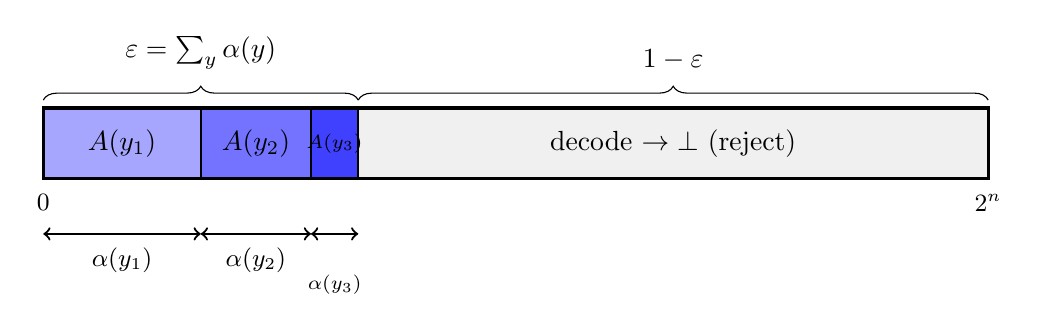
\begin{tikzpicture}[x=1cm, y=1cm]
  % Hash space outline
  \draw[very thick] (0,0) rectangle (12,0.9);

  % Acceptance regions (Shannon-optimal: width proportional to p_y)
  % Total accepted = epsilon = 4 (i.e., epsilon = 4/12 = 1/3 in this example)
  \fill[blue!35] (0,0) rectangle (2.0,0.9);    % A(y_1), p_1 = 0.50
  \fill[blue!55] (2.0,0) rectangle (3.4,0.9);  % A(y_2), p_2 = 0.35
  \fill[blue!75] (3.4,0) rectangle (4.0,0.9);  % A(y_3), p_3 = 0.15
  \fill[gray!12] (4.0,0) rectangle (12,0.9);   % reject region (noise)

  % Boundaries (redraw on top of fill)
  \draw[very thick] (0,0) rectangle (12,0.9);
  \draw[thick] (2.0,0) -- (2.0,0.9);
  \draw[thick] (3.4,0) -- (3.4,0.9);
  \draw[thick] (4.0,0) -- (4.0,0.9);

  % Region labels inside
  \node at (1.0, 0.45) {$A(y_1)$};
  \node at (2.7, 0.45) {$A(y_2)$};
  \node at (3.7, 0.45) {\scriptsize $A(y_3)$};
  \node at (8.0, 0.45) {decode $\to \bot$ (reject)};

  % Endpoint labels
  \node[below=2pt] at (0,0) {\small $0$};
  \node[below=2pt] at (12,0) {\small $2^n$};

  % Width annotations: alpha(y_i) = epsilon * p_{y_i}
  \draw[<->, thick] (0, -0.7) -- (2.0, -0.7);
  \node[below] at (1.0, -0.75) {\small $\alpha(y_1)$};
  \draw[<->, thick] (2.0, -0.7) -- (3.4, -0.7);
  \node[below] at (2.7, -0.75) {\small $\alpha(y_2)$};
  \draw[<->, thick] (3.4, -0.7) -- (4.0, -0.7);
  \node[below=10pt, font=\scriptsize] at (3.7, -0.75) {$\alpha(y_3)$};

  % Top braces: total accept (epsilon) and reject (1 - epsilon)
  \draw [decorate, decoration={brace, amplitude=5pt}] (0, 1.0) -- (4.0, 1.0);
  \node[above=6pt] at (2.0, 1.05) {$\varepsilon = \sum_y \alpha(y)$};

  \draw [decorate, decoration={brace, amplitude=5pt}] (4.0, 1.0) -- (12, 1.0);
  \node[above=6pt] at (8.0, 1.05) {$1 - \varepsilon$};
\end{tikzpicture}
\caption{Acceptance predicate partition of the $n$-bit hash space.
Each value $y \in Y$ is assigned an acceptance set $A(y)$ with
probability $\alpha(y) = |A(y)| / 2^n$.  Under Shannon-optimal
allocation $\alpha(y) = \varepsilon \cdot p_y$ (where $p_y =
\Pr[f(X) = y]$), region widths are proportional to value frequencies:
the dominant value $y_1$ occupies the largest region.  A hash falling
in $A(y)$ decodes to $y$; a hash outside the accepted region (total
measure $1 - \varepsilon$) decodes to $\bot$.  The Shannon-frequency
duality (\S\ref{subsec:acceptance}) holds because the same allocation
that minimizes the per-element bit cost ($-\log_2 \varepsilon + H(Y)$)
also makes the cipher value distribution match the latent value
distribution, defeating frequency analysis.}
\label{fig:acceptance-partition}
\end{figure}

\begin{remark}[XOR-scrambled decode]
The decode function applies a secret-derived XOR mask before checking
acceptance boundaries: $\dec(r)$ checks whether $r \oplus s_{\mathrm{key}}$
falls in the acceptance region for some $y$.  Without the scramble key, the
mapping from hash values to output values is pseudorandom; contiguous
acceptance regions in the scrambled space appear scattered in the raw hash
space.  This prevents an adversary observing hash outputs from inferring
which outputs correspond to which values, even if the acceptance regions are
contiguous.
\end{remark}

Different predicates give different space and construction-time trade-offs:
\begin{itemize}
\item \textbf{Prefix-free code.}
    $A(y) = \{c \in \{0,1\}^n : c \text{ starts with codeword}(y)\}$.
    Acceptance probability $\alpha(y) = 2^{-|\text{code}(y)|}$.
    Shannon-optimal when $|\text{code}(y)| \approx -\log_2 p_y$.
    This is the entropy cipher map construction.
\item \textbf{Threshold.}
    $A(y) = \{c : c < t(y)\}$ for thresholds $0 = t_0 < t_1 < \cdots$.
    Acceptance probability $\alpha(y) = (t_{y+1} - t_y) / 2^n$.
    Allows fine-grained control of per-value acceptance rates.
\item \textbf{Range partition.}
    Partition $[0, 2^n)$ into contiguous ranges $[l_y, l_y + w_y)$.
    Setting $w_y \propto p_y$ achieves Shannon-optimal allocation with
    uniform acceptance probability.
\end{itemize}

All three achieve the same space bound $-\log_2 \varepsilon + H(Y)$
bits per element when acceptance probabilities are Shannon-optimal
($\alpha(y) \propto p_y$).  They differ in construction time and
implementation simplicity.

\paragraph{Shannon-optimal allocation and frequency hiding.}
Setting $\alpha(y) \propto \Pr[f(X)=y]$ simultaneously achieves two
goals (\Cref{fig:acceptance-partition}).
First, it minimizes space: the per-element encoding cost
$-\log_2 \alpha(y) \approx -\log_2 p_y$ is the Shannon information content
of value $y$, and the average cost
$\sum_y p_y (-\log_2 p_y) = H(Y)$ is the entropy of the output
distribution.  Second, it hides value frequencies: noise queries (random
hash values) hit acceptance set $A(y)$ with probability
$\alpha(y) \propto p_y$---the same distribution as real queries.  An
adversary observing output values cannot distinguish whether a result came
from a real query or noise, because the output frequency profile is
identical in both cases.

These are not two independent optimizations that happen to coincide.
Shannon-optimal coding IS frequency hiding: matching the acceptance
distribution to the output distribution simultaneously minimizes space and
maximizes indistinguishability.  Any deviation from $\alpha(y) \propto p_y$
both wastes space (encoding rare values with fewer bits than their
information content requires) and leaks information (the frequency profile
of outputs differs between real and noise queries).

\subsection{Construction Algorithm}
\label{subsec:construction-alg}

\begin{algorithm}
\caption{Batch Cipher Map Construction}
\label{alg:singular-hash}
\begin{algorithmic}[1]
\Function{BuildCipherMap}{$M$, $A$, $h$, $\eta$}
    \Comment{$A$: acceptance predicate, $\eta$: target error rate}
    \State $m \gets |M|$
    \State $\ell \gets 0$
    \While{true}
        \State \text{Shuffle}$(M)$
            \Comment{random order for unbiased early stopping}
        \State $\text{fail} \gets 0$;\; $\text{pass} \gets 0$
        \For{$(x, y) \in M$}
            \State $\text{hash} \gets h(\ell) \oplus h(x)$
            \If{$\text{hash} \in A(y)$}
                \State $\text{pass} \gets \text{pass} + 1$
                \If{$\text{pass} \geq \lceil(1-\eta)\, m\rceil$}
                    \State \Return $\text{CipherMap}(h, A, \ell)$
                        \Comment{early accept}
                \EndIf
            \Else
                \State $\text{fail} \gets \text{fail} + 1$
                \If{$\text{fail} > \lfloor \eta\, m \rfloor$}
                    \State \textbf{break}
                        \Comment{early reject}
                \EndIf
            \EndIf
        \EndFor
        \State $\ell \gets \ell + 1$
    \EndWhile
\EndFunction
\end{algorithmic}
\end{algorithm}

Algorithm~\ref{alg:singular-hash} searches for a seed $\ell$ such that at most
$\lfloor \eta \cdot m \rfloor$ elements of $M$ fail the acceptance
predicate.  When $\eta = 0$, the first failure triggers rejection (the
exact case).  Query evaluation computes
$\fhat(c) = h(\ell) \oplus h(c)$ and decodes via $A$.

Two early-stopping rules avoid checking all $m$ elements:
\begin{itemize}
\item \textbf{Early reject:} if failures exceed $\lfloor \eta\, m \rfloor$,
    no remaining successes can help.
\item \textbf{Early accept:} if successes reach $\lceil (1-\eta)\, m \rceil$,
    the error budget is satisfied regardless of remaining elements.
\end{itemize}
Shuffling $M$ each iteration ensures both rules trigger as early as
possible: failures are not clustered at the end by a fixed ordering.

\subsection{Space Optimality}

\begin{theorem}[Information-theoretic space complexity]
\label{thm:space-optimal}
The batch construction has information-theoretic space complexity
\begin{equation}
(1-\eta)\bigl(-\log_2 \varepsilon + \mu\bigr) \text{ bits per element},
\end{equation}
where $\mu = H(Y)$ is the mean encoding length.  This is the information
content of the $(1-\eta)n$ correctly encoded elements.  When $\eta = 0$,
the bound matches the lower bound of Theorem~\ref{thm:lower-bound}.
\end{theorem}

\begin{proof}
\emph{Step 1: False negative reduction.}
When false negatives are permitted at rate $\eta$, only $(1-\eta)n$ of the
$n$ elements must decode correctly; the failing elements carry no
information about the latent function and contribute zero to the
information content of the construction.

\emph{Step 2: Per-element seed-table storage cost.}
For each correctly stored element $x_i$ with target value $y_i$, the
construction must record which of the $1/\alpha(y_i)$ candidate seeds
satisfies the acceptance constraint $h(\ell) \oplus h(x_i) \in A(y_i)$
(Definition~\ref{def:acceptance}).  Under the random oracle model with
Shannon-optimal allocation $\alpha(y) = \varepsilon \cdot p_y$
(proportional to value frequency, normalized so $\sum_y \alpha(y) =
\varepsilon$), the seed-table storage cost per element is
$-\log_2 \alpha(y_i) = -\log_2 \varepsilon - \log_2 p_y$ bits.  Per-element
storage costs sum across the $(1-\eta)n$ correctly encoded elements (by
independence of the per-element acceptance events under the random
oracle model).  We emphasise that this is the storage cost (bits to
record the chosen seed), separate from the construction-time cost
(number of seed trials, which scales as $1/\alpha(y_i)$ per element and
is analysed in \S\ref{subsec:tractability}).  Averaging the storage cost
over the value distribution gives
\[
\mathbb{E}_{y \sim p}\bigl[-\log_2 \alpha(y)\bigr]
\;=\; \mathbb{E}_{y \sim p}\bigl[-\log_2 \varepsilon - \log_2 p_y\bigr]
\;=\; -\log_2 \varepsilon \;+\; H(Y).
\]
The two terms have distinct interpretations: $-\log_2 \varepsilon$ is
the constant cost of distinguishing a valid encoding from one of the
$2^n(1-\varepsilon)$ noise-decoding bit strings, and $H(Y) = \mu$ is the
amortized cost of identifying \emph{which} value an encoding carries.
Choosing $\alpha(y) \propto p_y$ achieves the entropy lower bound on the
second term while pinning the first.

\emph{Step 3: Combining.}
Each correctly encoded element carries $-\log_2 \varepsilon + \mu$ bits of
information, and $(1-\eta)n$ such elements are encoded, giving total
information content $(1-\eta)n(-\log_2 \varepsilon + \mu)$ bits.
\end{proof}

\begin{remark}[Information-theoretic vs.\ physical storage]
\label{rem:physical-storage}
The $(1-\eta)$ factor is an information-theoretic statement about useful
content, not an automatic reduction in physical storage.  In the two-level
hash construction (Algorithm~\ref{alg:singular-hash}), the seed table
contains the same number of entries regardless of $\eta$: the $\eta n$
failing elements still occupy slots, but their seeds are ``don't cares.''
Physical storage matches the bound when the seed table is entropy-coded;
uncompressed storage is $-\log_2 \varepsilon + \mu$ bits per element
regardless of $\eta$.  The $\eta$ parameter primarily reduces construction
difficulty (fewer constraints to satisfy), not raw storage.
\end{remark}

\begin{corollary}[Asymptotic optimality]
When $\eta = 0$, the batch construction achieves $-\log_2 \varepsilon + H(Y)$
bits per element, matching the information-theoretic lower bound.
\end{corollary}

\subsection{Construction Time and Bucketing}
\label{subsec:tractability}

\begin{proposition}[Per-seed success probability]
\label{prop:construction-time}
For $m$ stored elements with acceptance predicate $A$ and target error rate
$\eta$, each element independently passes with probability $\alpha(y_i)$
under the random oracle model.  The number of failures $F$ follows a
Poisson binomial distribution, and the seed is accepted when
$F \leq \lfloor \eta m \rfloor$.

\emph{Special cases:}
\begin{itemize}
\item $\eta = 0$: $p = \prod_{i=1}^m \alpha(y_i)$ (all must pass).
\item Uniform $\alpha$:
    $p = \Pr[\mathrm{Bin}(m, 1-\alpha) \leq \lfloor \eta m \rfloor]$.
\end{itemize}
The expected number of seeds tried is $1/p$.
\end{proposition}

\begin{proof}
Under the random oracle model, the hash values $h(\ell) \oplus h(x_i)$ for
distinct $x_i$ are independent.  Element $x_i$ fails with probability
$1 - \alpha(y_i)$.  The failure count $F = \sum_i \mathbf{1}[\text{hash}_i
\notin A(y_i)]$ is a sum of independent Bernoulli variables.  The seed
is accepted when $F \leq \lfloor \eta m \rfloor$, giving the Poisson
binomial CDF.  For uniform $\alpha$, this reduces to the binomial CDF.
\end{proof}

The effect of $\eta > 0$ on construction time is dramatic.  For uniform
$\alpha$ and $m = 100$:

\begin{center}
\begin{tabular}{@{}llll@{}}
\toprule
$\alpha$ & $\eta = 0$ & $\eta = 0.01$ & $\eta = 0.05$ \\
\midrule
0.5 & $2^{100}$ & $2^{93}$ & $2^{74}$ \\
0.9 & $3.8 \times 10^4$ & $3.1 \times 10^3$ & $17$ \\
0.99 & 2.7 & 1.5 & 1.0 \\
\bottomrule
\end{tabular}
\end{center}

When $\eta$ exceeds the expected failure rate $1 - \alpha$, the binomial
tail concentrates and construction becomes near-certain on the first seed.
The transition is sharp: a few percent of tolerable error can reduce
construction time by tens of orders of magnitude.

\paragraph{Bucketed construction.}
The intractability of the global seed search is not inherent.  Partition
the $m$ elements into $k$ buckets (e.g., by
$h(x) \bmod k$) and find a separate seed $\ell_j$ for each bucket.

\begin{proposition}[Bucketed construction time ($\eta = 0$)]
\label{prop:bucketed}
With $k$ buckets of expected size $m/k$ and $\eta = 0$, the expected total
construction time is
\begin{equation}
T(k) = k \cdot \left(\frac{1}{\bar{\alpha}}\right)^{m/k},
\end{equation}
where $\bar{\alpha} = \bigl(\prod_i \alpha(y_i)\bigr)^{1/m}$ is the
geometric mean acceptance probability.
\end{proposition}

\begin{proof}
Each bucket has $m/k$ elements (in expectation).  The per-bucket success
probability is $\bar{\alpha}^{m/k}$ by
Proposition~\ref{prop:construction-time}.  Expected trials per bucket:
$(1/\bar{\alpha})^{m/k}$.  Summing over $k$ independent buckets gives the
result.
\end{proof}

The trade-off between construction time and space is controlled by $k$:

\begin{center}
\begin{tabular}{@{}llll@{}}
\toprule
Buckets $k$ & Seeds stored & Construction time & Space overhead \\
\midrule
1 (global) & 1 & $(1/\bar{\alpha})^m$ & $O(\log m) / m$ bits/elem \\
$\sqrt{m}$ & $\sqrt{m}$ & $\sqrt{m} \cdot (1/\bar{\alpha})^{\sqrt{m}}$
    & $O(\log m / \sqrt{m})$ bits/elem \\
$m$ (per-element) & $m$ & $m / \bar{\alpha}$ (linear)
    & $O(\log(1/\bar{\alpha}))$ bits/elem \\
\bottomrule
\end{tabular}
\end{center}

At $k = m$, each bucket has one element, construction is linear in $m$,
and the overhead is $\log_2(1/\bar{\alpha})$ bits per element for the
per-element seed---the same order as the hash width.  This is the regime
of practical perfect hash functions~\cite{belazzougui2009hash}.

An alternative construction uses perfect hash functions (PHFs) to assign
elements to slots in $O(m)$ time, avoiding the seed search entirely.  A PHF
maps the $m$ cipher keys to $m$ distinct slots; each slot stores the
XOR-masked value encoding.  Construction time drops from exponential in
bucket size to linear in $m$.  A reference implementation using a
RecSplit-family PHF~\cite{esposito2020recsplit} achieves $\sim$~713
documents per second on the full 20~Newsgroups corpus (18{,}266
documents, 58{,}903 words; 25.6~s wall-clock), compared to approximately
10 documents per second with the seed search construction.  Detailed
construction-time scaling appears in \S\ref{subsec:eval-20ng}.

\subsection{Instantiations}
\label{subsec:instantiations}

\subsubsection{Entropy Cipher Map}
\label{subsec:entropy-cipher-map}

The \emph{entropy cipher map} is the batch construction
(Algorithm~\ref{alg:singular-hash}) instantiated with a prefix-free
acceptance predicate.  It is the general batch cipher map for arbitrary
$f : X \to Y$, achieving Shannon-entropy-optimal value encoding.

\paragraph{Latent function.}
Arbitrary $f : X \to Y$ where $Y$ is finite.

\paragraph{Construction.}
Assign a prefix-free code $C_y \subseteq \{0,1\}^*$ for each $y \in Y$,
where the fraction of hash space covered by $C_y$ is proportional to
$\Pr_D[f(X) = y]$.  Find a seed $s$ (via two-level hashing,
\S\ref{subsec:tractability}) such that
\[
h(x \| s) \in C_{f(x)} \quad \text{for all } x \in X.
\]
Evaluation: compute $h(c \| s)$ and decode via the prefix-free code.

\paragraph{Two-level hash (practical algorithm).}
\begin{enumerate}
\item A primary hash maps $x$ to a bucket index $j \in \{0, \ldots, b-1\}$.
\item For each bucket, find a local seed $s_j$ such that $h(x \| s_j)$
    decodes to $f(x)$ for all $x$ in bucket $j$.
\item Store $s_j$ in a seed table $H[j]$.
\item Query: compute bucket $j$ (1~hash), evaluate $h(x \| H[j])$ and
    decode (1~hash).  Total: $O(1)$ hash operations.
\end{enumerate}

\paragraph{Mapping to cipher map abstraction.}
\begin{itemize}
\item $\fhat(c) = h(c \| H[\mathrm{bucket}(c)])$, total function.
\item $\enc(x, 0) = x$ (simplest version; $K(x)=1$).
\item $\dec(r) = y$ if $r \in C_y$ for some $y$, else $\bot$.
\end{itemize}

\paragraph{Parameter instantiation.}
\begin{center}
\begin{tabular}{@{}lll@{}}
\toprule
Parameter & Value & Justification \\
\midrule
$\eta$ & Tunable & Fraction of elements failing acceptance predicate \\
$\varepsilon$ & Code-dependent & Pr[random bits $\in \bigcup_y C_y$] \\
$\mu$ & $H(Y)$ & Shannon entropy of output distribution \\
$\delta$ & From code assignment & If $|C_y| \propto \Pr[f(X)=y]$,
    approaches uniform \\
Space & $-\log_2\varepsilon + H(Y)$ bits/element & \\
\bottomrule
\end{tabular}
\end{center}

\paragraph{Property status.}
Totality: \textbf{yes}.  Representation uniformity: \textbf{achievable}
(by assigning multiple codes proportional to output frequency).
Correctness: \textbf{yes} ($\eta \approx 0$, tunable via
Algorithm~\ref{alg:singular-hash}).  Composability:
\textbf{yes} (output is an $n$-bit string; serves as input to another
cipher map).

\begin{proposition}[Entropy cipher map space]
\label{prop:entropy-space}
The space per element of an entropy cipher map for $f : X \to Y$ with
output distribution $(p_y)_{y \in Y}$ equals
$-\log_2 \varepsilon + H(Y)$
bits, where $H(Y) = -\sum_y p_y \log_2 p_y$.
\end{proposition}

\begin{proof}
The term $-\log_2 \varepsilon$ is the per-element cost of distinguishing
signal from noise: each stored element requires that its hash prefix match a
valid codeword, which occurs with probability $\varepsilon$ for random
inputs.  The term $H(Y)$ is the expected code length under
Shannon-optimal prefix-free coding, which equals the entropy of the output
distribution by Shannon's source coding theorem~\cite{shannon1948mathematical}.  These two components are
additive because the noise-rejection bits and the value-encoding bits occupy
disjoint portions of the hash output.
\end{proof}

\begin{remark}[Set membership as a cipher map]
\label{rem:membership}
Set membership $\mathbf{1}_A : X \to \mathrm{Bool}$ is a cipher map
with $Y = \{\mathit{true}, \mathit{false}\}$.  The acceptance predicate
partitions hash space into $A(\mathit{true})$ and $A(\mathit{false})$,
with both outputs appearing as opaque bit strings.  Shannon-optimal
allocation sets $|A(\mathit{true})| \propto \Pr[x \in A]$ and
$|A(\mathit{false})| \propto \Pr[x \notin A]$.  For members, the seed
search ensures $h(\ell) \oplus h(x) \in A(\mathit{true})$.  For
non-members, the hash lands in $A(\mathit{false})$ with probability
$1 - \varepsilon$, providing both correct classification and
output-frequency hiding.  Space per element:
$-\log_2 \varepsilon + H(\mathrm{Bool})$ bits, where
$H(\mathrm{Bool}) = -p \log_2 p - (1\!-\!p) \log_2(1\!-\!p)$ for
$p = \Pr[x \in A]$.

The traditional Bloom filter~\cite{bloom1970space} tests membership but
reveals the raw Boolean result.  The cipher map version hides both the
input (via $\enc$) and the output (via the acceptance predicate), at the
cost of storing per-element seeds and accepting a noise-decode probability
$\varepsilon$.
\end{remark}


%% ============================================================
\section{Composition}
\label{sec:composition}

\subsection{Warm-Up: The AND Gate}
\label{subsec:and-gate}

Before proving the general composition theorem, we analyze a concrete case:
the AND gate operating on two independent Bernoulli Boolean values
$B_1, B_2$ with correctness probabilities $p_1 = 1-\eta_1$ and
$p_2 = 1-\eta_2$.

\begin{proposition}[AND gate correctness]
\label{prop:and-gate}
The correctness probability of $\mathrm{AND}(B_1, B_2)$ as an approximation
of $\mathrm{AND}(x_1, x_2)$ depends on the latent inputs:
\begin{center}
\begin{tabular}{@{}cccc@{}}
\toprule
$x_1$ & $x_2$ & $\mathrm{AND}(x_1,x_2)$ & $\Pr[\text{correct}]$ \\
\midrule
$1$ & $1$ & $1$ & $p_1 p_2$ \\
$1$ & $0$ & $0$ & $1 - p_1(1-p_2)$ \\
$0$ & $1$ & $0$ & $1 - p_2(1-p_1)$ \\
$0$ & $0$ & $0$ & $p_1 + p_2 - p_1 p_2$ \\
\bottomrule
\end{tabular}
\end{center}
\end{proposition}

\begin{proof}
We verify the $(1,0)$ case; the others are analogous.  When $x_1=1$,
$x_2=0$, the correct output is $0$.  The output is wrong ($=1$) only when
$B_1=1$ (correct, probability $p_1$) \emph{and} $B_2=1$ (incorrect,
probability $1-p_2$).  So
$\Pr[\text{wrong}] = p_1(1-p_2)$ and
$\Pr[\text{correct}] = 1 - p_1(1-p_2) = 1 - p_1 + p_1 p_2$.
\end{proof}

The output has a \emph{four-case correctness profile}: four distinct
correctness probabilities, one per input pair $(a, b) \in \{0,1\}^2$,
despite the Boolean output taking only two values.  Rather than tracking
all four cases separately, interval arithmetic propagates a bound
$[\min_{\text{cases}} p_{\text{correct}},\; \max_{\text{cases}} p_{\text{correct}}]$.
For AND with $p_1, p_2 \in (0.5, 1)$: minimum $p_1 p_2$ (case $(1,1)$);
maximum $p_1 + p_2 - p_1 p_2$ (case $(0,0)$).

\subsection{General Composition Theorem}

\begin{definition}[Re-randomization condition]
\label{def:re-randomization}
A composition $\ghat \circ \fhat$ satisfies the \emph{re-randomization
condition} when (i)~$\fhat$ and $\ghat$ are constructed with
independent operational sub-derivations of the master secret (automatic
under the random oracle model with distinct domain separators per
cipher map; see Remark~\ref{rem:master-vs-op}), and
(ii)~conditional on $\fhat$ producing a particular output, $\ghat$'s
correctness on that output is independent of whether $\fhat$ was
correct.  Operationally, this requires that the encoded output of
$\fhat$ is statistically indistinguishable from a freshly drawn cipher
value at $\ghat$'s input, so that $\ghat$'s acceptance behavior cannot
be correlated with $\fhat$'s error events.  Domain-separated sub-keys
suffice for (i); fresh per-call multiplicities $K(x) > 1$ or noise
injection between maps are mechanisms for (ii).
\end{definition}

\begin{theorem}[Composition correctness]
\label{thm:composition}
Let $\fhat$ be a cipher map for $f : X \to Y$ with correctness $\eta_f$,
and $\ghat$ a cipher map for $g : Y \to Z$ with correctness $\eta_g$.  Then
$\ghat \circ \fhat$ is a cipher map for $g \circ f$ with correctness
\begin{equation}
\eta_{g \circ f} \leq \eta_f + \eta_g - \eta_f \eta_g
  = 1 - (1 - \eta_f)(1 - \eta_g),
\end{equation}
with equality under the re-randomization condition
(Definition~\ref{def:re-randomization}).
\end{theorem}

\begin{proof}
The composition is incorrect when at least one map errs.  Let
$A = \{\fhat \text{ errs}\}$ and $B = \{\ghat \text{ errs}\}$.
By inclusion-exclusion,
$\Pr[A \cup B] = \Pr[A] + \Pr[B] - \Pr[A \cap B]$.
Note that the bound $\Pr[A \cup B]$ is pessimistic: it counts every
case in which at least one map errs as a composition error, but
occasional error cancellation occurs when $\fhat$ produces a wrong
intermediate value $y' \neq f(x)$ on which $\ghat$ nonetheless evaluates
to $g(f(x))$.  Such cancellations are rare in well-chosen codomains and
we do not attempt to credit them in the bound below.

\emph{Loose bound.}  Dropping $\Pr[A \cap B] \geq 0$ gives the union bound
$\eta_{g \circ f} \leq \eta_f + \eta_g$.

\emph{Under re-randomization.}
If the errors are independent ($\Pr[A \cap B] = \eta_f \eta_g$),
inclusion-exclusion gives
$\eta_{g \circ f} = \eta_f + \eta_g - \eta_f \eta_g
  = 1 - (1-\eta_f)(1-\eta_g)$.

In practice, $\fhat$ produces a specific encoding of $f(x)$, not a
uniformly random one.  If $\ghat$'s correctness depends on which encoding
it receives, the errors may be positively correlated
($\Pr[A \cap B] \leq \eta_f \eta_g$), making the bound
$\eta_f + \eta_g - \eta_f \eta_g$ conservative.
For specific circuits, the case-by-case interval arithmetic from
\S\ref{subsec:and-gate} gives tighter bounds.
\end{proof}

\begin{remark}[Garbage propagation]
When $\fhat$ produces an incorrect output on some input, the value fed to
$\ghat$ is effectively random.  Since $\ghat$ is a total function, it
produces \emph{some} output on this random input, which is correct with
probability at most $\varepsilon_g$ (the noise-decode probability of
$\ghat$).  Thus the bound
$\eta_{\mathrm{total}} \leq \eta_f + \eta_g - \eta_f \eta_g$ is an upper
bound; the actual error rate may be marginally lower due to accidental
correctness on garbage inputs.  For small $\eta_f, \eta_g$, this
distinction is negligible.
\end{remark}

\subsection{Composition Chains}

\begin{corollary}[Chain composition]
\label{cor:chain}
For a chain of $m$ cipher maps $\fhat_1, \ldots, \fhat_m$:
\begin{equation}
\eta_{\mathrm{total}} \leq 1 - \prod_{i=1}^{m}(1 - \eta_i),
\end{equation}
with equality under the re-randomization condition
(Definition~\ref{def:re-randomization}) applied pairwise along the
chain.  If all $\eta_i = \eta$:
\begin{equation}
\eta_{\mathrm{total}} \leq 1 - (1-\eta)^m \approx m\eta
\quad \text{for small } \eta.
\end{equation}
\end{corollary}

\begin{proof}
By induction on Theorem~\ref{thm:composition}.  The base case $m=2$ is the
theorem.  For the inductive step, the composition of $m-1$ maps has
correctness bounded by $1 - \prod_{i=1}^{m-1}(1-\eta_i)$; composing with
$\fhat_m$ and applying Theorem~\ref{thm:composition} again gives
$\eta_{\mathrm{total}} \leq 1 - \prod_{i=1}^{m-1}(1-\eta_i) \cdot (1-\eta_m)
= 1 - \prod_{i=1}^m (1-\eta_i)$.
The approximation follows from $\ln(1-\eta) \approx -\eta$ for small
$\eta$, giving $(1-\eta)^m \approx e^{-m\eta} \approx 1 - m\eta$.
\end{proof}

\begin{example}
A circuit of 100 cipher maps each with $\eta = 10^{-6}$:
$\eta_{\mathrm{total}} \leq 1 - (1-10^{-6})^{100} \approx 10^{-4}$
(equality under re-randomization).
\end{example}

\subsection{Error Accumulation by Gate Type}

For specific circuits, the AND gate analysis
(Proposition~\ref{prop:and-gate}) can be extended to OR, NOT, and arbitrary
Boolean gates.  Each gate type induces a different case table.  Rather than
tracking exact correctness per case, interval arithmetic propagates bounds:
at each gate, compute $[\eta_{\min}, \eta_{\max}]$ from the input intervals.
This gives input-dependent bounds tighter than the worst-case
Theorem~\ref{thm:composition}.


%% ============================================================
\section{Representation Uniformity and Encoding Granularity}
\label{sec:uniformity}

We measure representation uniformity using total variation distance $\TV$,
which bounds the distinguishing advantage of any statistical test.
We use TV rather than max-divergence ($D_\infty$) because the constructions
are designed around frequency equalization, which naturally yields TV bounds.

\subsection{The Encoding Granularity Principle}
\label{subsec:granularity}

Representation uniformity is defined \emph{per cipher map}: the
\emph{encoding granularity} is the domain type $X$, and uniformity applies
to the distribution over encodings of individual elements of $X$.  What
correlations are hidden depends on what is encoded as a unit.  Consider
encrypting a pair of Boolean values $(a, b)$ where $a$ and $b$ are
correlated.

\begin{description}
\item[Component-wise encoding ($p=1$).]
Encode $a$ and $b$ as separate cipher values.  Each component's marginal
distribution is $\delta$-close to uniform, but joint correlations leak.

\item[Pair-wise encoding ($p=2$).]
Encode $(a, b)$ as a single cipher value.  The distribution over pair
encodings is $\delta$-close to uniform; correlations between $a$ and $b$ are
hidden.  Cost: domain is $\{0,1\}^2$ (4 elements) rather than $\{0,1\}$
(2 elements); space per encoding grows.

\item[Whole-state encoding ($p=k$).]
Encode the entire program state as one cipher value.  All correlations are
hidden.  Cost: domain is the full state space, typically prohibitive.
\end{description}

\begin{definition}[Entanglement parameter]
For a system encoding $k$ correlated Boolean values, the \emph{entanglement
parameter} $p$ is the number of values encoded as a single unit.  The system
has type $\mathrm{cipher}(\{0,1\}^p)^{k/p}$, where each block of $p$ bits
is encoded jointly.
\end{definition}

\begin{proposition}[Granularity and privacy]
\label{prop:granularity}
Let $\fhat$ be a cipher map for $f : X_1 \times X_2 \to Y$ with
representation uniformity $\delta$.  Then the marginal distribution of
$\enc((x_1, x_2), k)$ over random $(x_1, x_2) \sim D$ and random $k$ is
$\delta$-close to uniform, and the joint distribution of $(x_1, x_2)$ is
hidden up to $\delta$.

Conversely, let $\fhat_1, \fhat_2$ be independent cipher maps for
$f_1 : X_1 \to Y_1$ and $f_2 : X_2 \to Y_2$, each with representation
uniformity $\delta$.  Then each marginal cipher value is $\delta$-close to
uniform, but correlations between $x_1$ and $x_2$ are \textbf{not hidden},
even when $\delta = 0$.
\end{proposition}

\begin{proof}
The first part follows directly from Definition~\ref{def:rep-uniformity}
applied to the joint cipher map.  For the second part: even with $\delta=0$
(perfect marginal uniformity), $\enc_i$ is injective for each fixed $k_i$.
The joint distribution of $(\enc_1(x_1, k_1), \enc_2(x_2, k_2))$ is
therefore a bijective image of the joint distribution of
$((x_1, k_1), (x_2, k_2))$, preserving all statistical dependence between
$x_1$ and $x_2$.  An adversary observing $N$ draws can estimate this joint
distribution and recover the correlation structure of $(x_1, x_2)$.
\end{proof}

\begin{remark}[Granularity trade-offs in adjacent frameworks]
The space-vs-correlation-hiding trade-off via the entanglement parameter
$p$ has analogues in oblivious RAM and private information retrieval.
ORAM constructions trade access-pattern hiding against per-access
overhead (polylogarithmic in storage size); PIR constructions trade
query unlinkability against communication and server work (one server
or computational PIR pays for unlinkability with cryptographic
overhead, multi-server information-theoretic PIR pays with replication).
The cipher map granularity knob is the analogous trade-off in the
parameterized-leakage setting: hiding the joint distribution of $k$
correlated values requires storage growing as $|Y|^k$, but obviates the
per-access protocols ORAM and PIR rely on.  Companion
work~\cite{towell2026maxconf} treats the granularity lever in detail
within the entropy-ratio framework.
\end{remark}

\subsection{Compositional Leakage}
\label{subsec:comp-leakage}

Even when each cipher map has uniform marginal output, composing multiple
cipher maps on a shared input leaks the correlation structure of the latent
functions.  Consider cipher maps $\fhat_1 : \{0,1\}^n \to \{0,1\}^n$ and
$\fhat_2 : \{0,1\}^n \to \{0,1\}^n$ for latent $f_1 : X \to Y$ and
$f_2 : X \to Z$, each with Shannon-optimal acceptance predicates.
Individually, the outputs $\hat{y}$ and $\hat{z}$ are uniform.  But the
untrusted machine observes both $\hat{y} = \fhat_1(c)$ and
$\hat{z} = \fhat_2(c)$ for the same cipher value~$c$.  Since $\fhat_1$ and
$\fhat_2$ are deterministic, the pair $(\hat{y}, \hat{z})$ is a
deterministic function of~$c$, and the joint distribution of
$(\hat{y}, \hat{z})$ preserves the latent correlation between $f_1$ and
$f_2$ (Proposition~\ref{prop:granularity}).

If a third cipher map $\fhat_3$ takes this correlated pair as input, its
output inherits the non-uniformity: $\fhat_3$ was constructed assuming a
design distribution over its inputs, but the actual input distribution
reflects latent correlations.  The output $\hat{w}$ is non-uniform even if
$\fhat_3$'s acceptance predicate is Shannon-optimal for the marginal
distribution of~$W$.  Every observable correlation between cipher values
carries information about the latent data.

\paragraph{Mitigation strategies.}
Two approaches exist, both costly:

\begin{description}
\item[Build the composition directly.]
Construct a single cipher map for the composed function
$g(x) = f_3(f_1(x), f_2(x))$ as one batch construction.  The untrusted
machine sees only the cipher input $\hat{x}$ and the final cipher output
$\hat{w}$; no intermediate values are exposed.  This eliminates
compositional leakage entirely but costs $O(|X| \cdot (-\log_2 \varepsilon
+ H(W)))$ space and exponential construction time---the entire program is
a single lookup table.

\item[Compose components and inject noise.]
Keep the practical component-wise evaluation ($\fhat_1$, $\fhat_2$,
$\fhat_3$ as separate cipher maps) and add $R$ noise queries for every
$N$ real queries.  By totality, noise and real queries are
indistinguishable to~$U$.  The adversary's estimates of pairwise
correlations have variance $O(1/N)$; mixing with $R \gg N$ noise pairs
dilutes the signal proportionally.  This costs bandwidth rather than space.
\end{description}

The fundamental trade-off: constructing the composition as a single cipher
map gives full privacy at the cost of space and construction time.
Composing component cipher maps is practical but leaks intermediate
correlations.  Noise injection is an intermediate strategy that trades
bandwidth for privacy.  The entanglement parameter $p$ controls the
granularity of this trade-off.

\paragraph{Honest limitations.}
\begin{enumerate}
\item Marginal uniformity says nothing about joint distributions.
\item Compositional leakage is inherent in component-wise evaluation;
    only joint encoding or noise injection can mitigate it.
\item Equality pattern leakage is fundamental: any deterministic encoding
    leaks the equality pattern of its inputs.  Multiple representations
    ($K(x) > 1$) reduce but do not eliminate this.  The next subsection
    quantifies this leakage as a function of instance count and
    acceptance allocation, and analyzes randomized encoding as a
    defense.
\end{enumerate}


%% ============================================================
%% [INTEGRATION 2026-05-07] New subsection §8.3
\subsection{Multi-Instance Composition Leakage}
\label{subsec:multi-instance}

The previous subsection identified equality-pattern leakage as
fundamental for deterministic encodings.  We now quantify it precisely
for the case of \emph{multi-instance composition}: the same latent
function $f : X \to Y$ encoded as $t$ cipher maps
$\fhat_1, \ldots, \fhat_t$, all observed by the same untrusted machine.
This deployment pattern arises whenever the same data is published
multiple times under different keys, when a cipher map is updated and
both versions remain accessible, or when an attacker collects
observations across multiple cipher map snapshots.

\subsubsection*{The coincidence oracle}

Consider $t$ cipher maps $\fhat_1, \ldots, \fhat_t$ for the same $f$
under independent secret seeds (so that filler-query outputs are
independent across instances by the random-oracle assumption), with
acceptance partitions $\{\alpha_i(y)\}_{y \in Y}$.  Under canonical
encoding ($K(x) = 1$ per value) and $\eta = 0$, members produce
identical decoded values across instances; non-members produce
independent decoded draws.  The simplest attacker, the
\emph{coincidence oracle}, predicts ``in-domain'' iff
$\dec_1(\fhat_1(c)) = \cdots = \dec_t(\fhat_t(c))$ and the common
decoded value is not~$\bot$.

\begin{theorem}[Coincidence-oracle accuracy]
\label{thm:coincidence-oracle}
Let $\fhat_1, \ldots, \fhat_t$ be canonical cipher maps for the same
latent function $f : X \to Y$ under independent secret seeds, each
with its own encoder $\enc_i$, decoder $\dec_i$, and acceptance
partition $\{\alpha_i(y)\}_{y \in Y}$, with $K(x) = 1$ for all $x$
(canonical encoding) and $\eta = 0$ (exact correctness).  Assume the
codec is public (the acceptance predicates $A_i$ are known to $U$).
Then under balanced class prior $\pi = 1/2$ between members
($x \in \mathrm{dom}(f)$ with $f(x) \in Y$) and non-members (filler queries),
the coincidence-oracle attacker's classification accuracy is
\begin{equation}
\mathrm{accuracy}(t)
\;=\; 1 \;-\; \tfrac{1}{2} \sum_{y \in Y} \prod_{i=1}^{t} \alpha_i(y).
\label{eq:coincidence-bound}
\end{equation}
For homogeneous instances (same partition $\alpha$ across all $i$):
\begin{equation}
\mathrm{accuracy}_{\mathrm{hom}}(t)
\;=\; 1 \;-\; \tfrac{1}{2} \sum_{y \in Y} \alpha(y)^t.
\label{eq:coincidence-homogeneous}
\end{equation}
\end{theorem}

\begin{proof}
We compute the attacker's conditional accuracy on each class, then
combine at the balanced prior.

\emph{Members.}
For a member $x \in \mathrm{dom}(f)$ with $f(x) \in Y$, the trusted side
publishes one cipher value per instance, $c_i = \enc_i(x, 0)$ (the
single multiplicity index under $K(x) = 1$).  Under $\eta = 0$ each
cipher map decodes correctly, so
$\dec_i(\fhat_i(c_i)) = f(x)$ for every~$i$.  All $t$ decoded values
equal the common value $f(x) \in Y$; the coincidence-oracle predicate
``all match a common $y \in Y$'' is satisfied, and the attacker
correctly predicts ``in-domain'':
$\Pr[\text{predict in} \mid \text{member}] = 1$.

\emph{Non-members (filler).}
For a non-member input, the $t$ cipher values $(c_1, \ldots, c_t)$
fed to the cipher maps are not stored in any instance.  Under the
random oracle model with independent per-instance seeds, the hash
outputs $\fhat_i(c_i)$ are independent across $i$ and each uniform
on~$\B^n$.  The per-instance decoded value distribution is therefore
$\Pr[\dec_i(\fhat_i(c_i)) = y] = \alpha_i(y)$ for each $y \in Y$
and $\Pr[\dec_i(\fhat_i(c_i)) = \bot] = 1 - \varepsilon_i$, with
events independent across instances.  The attacker's predicate
explicitly excludes the common-$\bot$ case (it requires the common
value to lie in $Y$), so by independence,
\[
\Pr[\text{predict in} \mid \text{filler}]
  = \sum_{y \in Y} \Pr\!\left[\bigwedge_{i=1}^{t} \dec_i(\fhat_i(c_i)) = y\right]
  = \sum_{y \in Y} \prod_{i=1}^{t} \alpha_i(y).
\]
All other outcomes (some pair disagrees, or all agree on $\bot$)
correctly classify the input as ``not in-domain''.

\emph{Combining at $\pi = 1/2$.}
\begin{align*}
\mathrm{accuracy}
  &= \pi \cdot \Pr[\text{predict in} \mid \text{member}]
   + (1 - \pi) \cdot \Pr[\text{predict not in} \mid \text{filler}] \\
  &= \tfrac{1}{2} \cdot 1
   + \tfrac{1}{2} \left(1 - \sum_{y \in Y} \prod_{i=1}^{t} \alpha_i(y)\right)
   = 1 - \tfrac{1}{2} \sum_{y \in Y} \prod_{i=1}^{t} \alpha_i(y).
\end{align*}
The homogeneous case follows by setting $\alpha_i = \alpha$ for
all~$i$, giving $\prod_i \alpha_i(y) = \alpha(y)^t$.
\end{proof}

\begin{remark}[General class prior and threat model]
\label{rem:coincidence-prior}
For general prior $\pi \in (0, 1)$, the same calculation gives
$\mathrm{accuracy}(t, \pi) = 1 - (1 - \pi) \sum_y \prod_i \alpha_i(y)$
when the coincidence-oracle rule is preferred to the trivial
``always predict not in domain'' rule (which has accuracy $1 - \pi$).
The crossover is at $(1 - \pi) \sum_y \prod_i \alpha_i(y) = \pi$;
for $\pi$ very small the coincidence-oracle rule loses to trivial,
but at any $\pi \geq \tfrac{1}{2}$ the bound \eqref{eq:coincidence-bound}
applies.  The public-codec assumption is essential: under a private
codec, the attacker cannot apply $\dec_i$ and must fall back on the
weaker pattern-coincidence attacker analyzed in
Proposition~\ref{prop:rand-encoding}.
\end{remark}

\paragraph{Empirical verification.}
A homogeneous sweep across five acceptance predicates and $t \in \{1,
2, 3, 4, 5\}$ (codec-controlled retrieval, balanced class prior,
$|S| = 2000$, $|Y| = 8$, 5000 evaluation queries per class per cell)
finds $24$ of $25$ cells with the predicted accuracy from
\eqref{eq:coincidence-homogeneous} inside the empirical Wilson 95\%
confidence interval; the single miss is at $0.003$ absolute sampling
noise.  Reported in \S\ref{subsec:eval-codec-security}.

\subsubsection*{Geometric corollary: \texorpdfstring{$t$}{t}-dependent allocation}

For homogeneous instances, $\sum_y \alpha(y)^t$ is dominated by
$(\max_y \alpha(y))^t$ as $t$ grows.  The codec choice minimizing
multi-instance coincidence-oracle leakage at large $t$ is therefore
the one minimizing $\max_y \alpha(y)$.  At fixed $\varepsilon = \sum_y
\alpha(y)$, this is the \emph{uniform} partition $\alpha(y) =
\varepsilon / |Y|$.

\begin{corollary}[$t$-dependent acceptance allocation]
\label{cor:t-dependent}
Among acceptance partitions with fixed $\varepsilon$:
\begin{itemize}
\item \textbf{$t = 1$ optimum:}  $\alpha(y) \propto p_y$ (Shannon-optimal
    allocation, \S\ref{subsec:acceptance}) minimizes single-instance
    leakage by matching real and noise frequency profiles.
\item \textbf{$t \geq 2$ shared-$f$ optimum:}  $\alpha(y) =
    \varepsilon / |Y|$ (uniform allocation) minimizes
    coincidence-oracle leakage by equalizing the geometric tail of the
    non-member distribution.
\end{itemize}
\end{corollary}

The two regimes pull in opposite directions when $f$ has skewed value
distribution.  For $|Y| = 8$ with a Zipf $p_y$ (skew parameter $s = 1$),
the Shannon-optimal Huffman partition gives $\max_y \alpha(y) \approx
0.5$ (the dominant value claims half the codespace), while uniform
gives $\max_y \alpha(y) = 1/8 = 0.125$.  At $t = 5$, uniform's
coincidence-oracle accuracy is $\approx 0.9999$ while the Shannon-optimal
Huffman partition gives $\approx 0.984$.  The Shannon-optimal partition
that wins at $t = 1$ leaks $\approx 16\times$ more under shared-$f$
multi-instance composition than the uniform partition.

\paragraph{Implication for deployment.}  The acceptance predicate is
not chosen on purely Shannon-optimal grounds.  A deployment publishing
a single cipher map should use $\alpha(y) \propto p_y$.  A deployment
publishing $t \geq 2$ instances over the same $f$ under independent
seeds should either use the uniform allocation, sacrificing
single-instance indistinguishability for multi-instance robustness, or
apply the randomized-encoding defense below.

\subsubsection*{Randomized encoding as a defense}

The coincidence oracle exploits the equality pattern of canonical
encoding.  Property~2 already permits $K(x) > 1$ (homophonic
substitution) as a representation-uniformity mechanism; we now
quantify it as a defense against the multi-instance attacker.

\begin{definition}[Randomized encoding]
\label{def:rand-encoding}
A cipher map uses \emph{randomized encoding} if the encoder samples
$k$ uniformly from $\{0, \ldots, K(x) - 1\}$ at each query and emits
$\enc(x, k)$.  Across instances, the per-query sample $k$ values are
independent.
\end{definition}

\begin{definition}[Pattern-coincidence and decode-coincidence attackers]
\label{def:pattern-decode-attackers}
Given $t$ cipher map instances $\fhat_1, \ldots, \fhat_t$ for the
same latent function $f$ under independent seeds and a probe
$\mathbf{c} = (c_1, \ldots, c_t)$ constructed by the trusted side as
$c_i = \enc_i(x, k_i)$ for a candidate input $x$:
\begin{description}
\item[Pattern-coincidence attacker (private-codec threat).]  Observes
    the raw cipher map outputs $\mathbf{M} = (\fhat_1(c_1), \ldots,
    \fhat_t(c_t)) \in (\B^n)^t$ and predicts ``in-domain'' iff all
    $t$ are equal as bit strings: $\fhat_1(c_1) = \cdots =
    \fhat_t(c_t)$.  Does not invoke $\dec_i$.
\item[Decode-coincidence attacker (public-codec threat).]  Observes
    the decoded values $\mathbf{D} = (\dec_1(\fhat_1(c_1)), \ldots,
    \dec_t(\fhat_t(c_t)))$ and predicts ``in-domain'' iff all $t$
    decoded values agree on a common value in $Y$.  Requires
    knowledge of the per-instance acceptance predicates.
\end{description}
\end{definition}

\begin{proposition}[Randomized-encoding defense, two threat models]
\label{prop:rand-encoding}
Let $\fhat_1, \ldots, \fhat_t$ be cipher maps for $f$ under
randomized encoding with multiplicity $K(x) \geq 1$ (each $\enc_i$
samples $k_i$ uniformly from $\{0, \ldots, K(x) - 1\}$ at every
query) and $\eta = 0$ (exact correctness).  Write $|A_i(y)|$ for
the size in bit strings of the value-$y$ acceptance region in
instance $i$, and assume the construction \emph{saturates} each
acceptance region: every bit string in $A_i(y)$ is reachable as
$\fhat_i(c)$ for some member cipher value $c$ encoding a value-$y$
plaintext (this holds, e.g., for Huffman codespace classes where
$K(x)$ equals the codespace class size $2^{n - \ell_{f(x)}}$).  Then
under the random oracle model with independent seeds:

\textbf{Pattern-coincidence (private codec).}
Conditional on $f(x) = y$,
\[
\Pr[\text{predict in} \mid \text{member, } f(x) = y]
  \;=\; \prod_{i=2}^{t} \frac{1}{|A_i(y)|},
\qquad
\Pr[\text{predict in} \mid \text{filler}]
  \;=\; \frac{1}{2^{n(t-1)}}.
\]
Increasing $|A_i(y)|$ via larger multiplicity $K(x)$ cuts the
in-domain coincidence probability by a factor of $|A_i(y)|^{t-1}$
relative to canonical encoding ($K(x) = 1$ gives $|A_i(y)| = 1$ and
$\Pr[\text{predict in} \mid \text{member}] = 1$).

\textbf{Decode-coincidence (public codec).}
The decoded value distribution is invariant under the
canonical-vs-randomized choice (every pattern in $A_i(y)$ decodes to
$y$ regardless of which is sampled).  Accuracy equals the
coincidence-oracle bound \eqref{eq:coincidence-homogeneous} of
Theorem~\ref{thm:coincidence-oracle}.
\end{proposition}

\begin{proof}
\emph{Pattern-coincidence, member.}
Fix a member $x$ with $f(x) = y$.  Each instance $i$ samples
$k_i \sim \mathrm{Unif}(\{0, \ldots, K(x) - 1\})$ and emits cipher
value $c_i = \enc_i(x, k_i)$.  Under $\eta = 0$, $\fhat_i(c_i) \in
A_i(y)$ for every $i$ (correctness, Property~3).  Under the random
oracle model with independent seeds and the saturation assumption,
the specific pattern $\fhat_i(c_i) \in A_i(y)$ chosen by instance
$i$ is uniformly distributed on the $|A_i(y)|$ patterns and
statistically independent across instances.  The probability that
all $t$ patterns coincide is the probability that instances
$2, 3, \ldots, t$ each match the pattern fixed by instance~$1$:
$\prod_{i=2}^{t} 1/|A_i(y)|$.

\emph{Pattern-coincidence, filler.}
For a filler input, each $\fhat_i(c_i)$ is uniform on $\B^n$ under
the random oracle model with independent seeds, and independent
across instances.  Then $\Pr[\text{all equal}] = \sum_{p \in \B^n}
(2^{-n})^t = 2^{n} \cdot 2^{-nt} = 2^{-n(t-1)}$.

\emph{Decode-coincidence.}
The decoded value $\dec_i(\fhat_i(c_i))$ depends only on which
acceptance set $A_i(y)$ contains $\fhat_i(c_i)$, not on the specific
pattern within that set.  Replacing the canonical sample
$\enc_i(x, 0)$ with the randomized $\enc_i(x, k_i)$ changes which
pattern in $A_i(y)$ is observed for member queries but not
\emph{which} acceptance set is hit; the decoded value marginals
are therefore identical to the canonical case.
Theorem~\ref{thm:coincidence-oracle}'s accuracy formula
\eqref{eq:coincidence-homogeneous} applies verbatim.
\end{proof}

\begin{remark}[Member coincidence under Huffman]
\label{rem:huffman-member-coincidence}
For a homogeneous Huffman codec with codeword lengths $\ell_v
\approx -\log_2 p_f(v)$ over a value distribution $p_f$, the
saturation assumption holds with $|A_i(v)| = 2^{n - \ell_v}$.
Marginalizing the member coincidence over $p_f$:
\[
\Pr[\text{predict in} \mid \text{member}]
  = \sum_{v} p_f(v) \cdot 2^{-(n - \ell_v)(t-1)}
  = 2^{-n(t-1)} \sum_v p_f(v) \cdot 2^{\ell_v(t-1)}.
\]
For $t = 2$ this reduces to $|Y| / 2^n$ (each summand contributes
$\approx 1$ under $2^{\ell_v} \approx 1/p_f(v)$).  For $t > 2$ the
summand $p_f(v) \cdot 2^{\ell_v(t-1)} \approx p_f(v)^{2-t}$ is
dominated by the rarest values and grows with $t$; the closed form
no longer collapses but remains tractable numerically.  Empirical
values appear in \S\ref{subsec:eval-codec-security}.
\end{remark}

\paragraph{Empirical verification.}
A sweep at $|S| = 1000$, $|Y| = 8$, $n = 4$~bits, codec-controlled
retrieval shows that randomized encoding reduces pattern-coincidence
accuracy from $1.000$ (canonical) to $0.699$ (randomized) for the
Huffman partition at $t = 4$, and to $0.543$ at $n = 5$~bits.
Decode-coincidence accuracy is unaffected by the encoding mode,
confirming the threat-model distinction.  Marginal output distribution
at $t = 1$ is identical between canonical and randomized encoding to
within $0.001$, confirming the defense is free in the single-instance
regime.  Reported in \S\ref{subsec:eval-codec-security}.

\paragraph{Honest limitations.}
\begin{enumerate}
\item Randomized encoding requires the codec (the acceptance
    predicate) to remain private.  When the codec is published or
    recoverable from queries, decode-coincidence applies and
    randomized encoding provides no protection.
\item The defense incurs space cost only when $\kappa(y) > 1$, which
    requires acceptance predicates with codespace slack.  The Dense
    partition ($\alpha(y) = 1/|Y|$, saturated) has $\kappa(y) = 1$ for
    all $y$ and gets no benefit from randomized encoding.
\item The decode-coincidence accuracy formula
    \eqref{eq:coincidence-homogeneous} still applies under the
    public-codec threat; the only structural defenses in that regime
    are the $t$-dependent allocation of
    Corollary~\ref{cor:t-dependent} and the encode-different-$f$-per-instance
    deployment recommended in \S\ref{subsec:eval-codec-security}.
\end{enumerate}
%% [/INTEGRATION 2026-05-07]


%% ============================================================
\section{Discussion}
\label{sec:discussion}

\subsection{Relationship to the Bernoulli Model}

The correctness parameter $\eta$ of a cipher map corresponds directly to the
error rate in a Bernoulli approximation.  A cipher map with correctness
$\eta$ induces a Bernoulli approximation of the latent function $f$: for
each $x \in X$,
$\Pr[\dec(\fhat(\enc(x,k))) \neq f(x)] = \eta(x)$,
where the failing elements are deterministic for a given seed.

The composition bound
$\eta_{g \circ f} \leq 1 - (1-\eta_f)(1-\eta_g)$
(equality under the re-randomization condition,
Definition~\ref{def:re-randomization})
is the standard error accumulation for independent Bernoulli events,
identical to the formula derived in the noisy gates framework for AND gates
over Bernoulli Booleans.  This is not coincidental: a cipher map \emph{is} a
Bernoulli approximation, viewed through the lens of hash-based total
functions.

The Bernoulli framework organizes approximation into a layered type hierarchy:
$\mathrm{Bool} \to \mathrm{Set} \to \mathrm{Map} \to \mathrm{Relation} \to
\mathrm{Type}$, where each level inherits the error model from the level
below.  The formalism presented here covers maps ($X \to Y$); relations and
algebraic types (sum types, product types) require the extensions developed in
the Bernoulli relations and algebraic types work~\cite{bernoulli-types}.
The BHF (Bernoulli Hash Function) construction from that framework is the
optimal cipher map for the batch strategy: it achieves the
$-\log_2 \varepsilon + H(Y)$ lower bound with $O(1)$ query time.

\subsection{Algebraic Structure}

The cipher map abstraction relates to algebraic concepts from the theory of
monoid homomorphisms.  The decoding function $\dec$ is (by construction) a
left inverse of $\enc$, and for cipher maps that preserve algebraic
structure (e.g., the trapdoor Boolean algebra), $\dec$ is a homomorphism
from the cipher monoid to the latent monoid---but only up to the
equivalence $c_1 \sim c_2 \iff \dec(c_1) = \dec(c_2)$.  The quotient
$\{0,1\}^n / {\sim}$ is isomorphic to the latent structure.

We note this connection but do not develop it further.  The category-theoretic
framing (cipher functors lifting monoids to cipher monoids) is a natural
extension but requires careful treatment of the approximate setting: the
functor laws hold exactly on the quotient but only approximately on
representatives.

\subsection{Online Construction}
\label{subsec:online}

The batch construction developed in \S\ref{sec:batch} requires knowing the
domain $X$ and function $f$ at construction time.  An alternative
\emph{online} strategy encodes sets incrementally via bitwise OR of
per-element hashes, with no seed search.  Union, intersection, and
complement reduce to bitwise OR, AND, and NOT; union is exact but
intersection and complement are approximate (cross-element hash collisions
and the pigeonhole principle, respectively).  This approach---the
\emph{trapdoor Boolean algebra}---is developed in a companion
paper~\cite{bernoulli-types}.  The batch and online strategies offer
complementary trade-offs: batch achieves information-theoretically optimal
space with tunable correctness; online enables incremental construction and
algebraic composition at the cost of space exponential in set size.

\subsection{Bounded Composition as a Security Feature}
\label{subsec:bounded-composition}

A cipher map composition $\cipherS{g}{s} \circ \cipherS{f}{s}$ stays
within the cipher space $\cipherS{\cdot}{s}$ indefinitely: there is no
construction-imposed limit on chain length under a single secret.  But
when secrets are rotated to mitigate accumulating leakage, a different
picture emerges.  The companion cipher rekeying
paper~\cite{towell2026rekeying} introduces a rekeying functor
$r_{s_i \to s_{i+1}} : \cipherS{X}{s_i} \to \cipherS{X}{s_{i+1}}$,
which transports cipher values across secret boundaries while preserving
latent meaning.  An $n$-step rekeying chain
\[
\cipherS{X}{s_0} \xrightarrow{r_{s_0 \to s_1}}
\cipherS{X}{s_1} \xrightarrow{r_{s_1 \to s_2}}
\cdots \xrightarrow{r_{s_{n-1} \to s_n}}
\cipherS{X}{s_n}
\]
admits the bound $H(X \mid \mathcal{V}) \geq H(X) - \log_2(n+1)$
where $\mathcal{V}$ is the adversary's view of all intermediate cipher
values~\cite[Thm.~7.1]{towell2026rekeying}: each rekeying step costs at
most one bit of latent entropy.

This couples a security guarantee to a complexity restriction.  The
trusted machine's pre-provisioned set of rekeying maps determines an
upper bound on chain length: programs whose composition depth depends
on input size cannot be expressed unless the trusted machine refreshes
the rekeying budget on demand.  In particular, the framework as
described here is not Turing-complete: it captures bounded-depth
straight-line composition (the typical $n = 2$ to $5$ regime of
encrypted search, classification cascades, or fixed-depth circuits) but
not unbounded recursion or input-dependent loops.

We frame this as a feature rather than a limitation.  Sub-Turing
computation models have a long history in security
contexts---capability machines bound resource use, total functional
languages exclude non-termination, structurally recursive type theories
exclude unbounded fixpoints---each trading expressivity for static
guarantees.  Cipher rekeying provides the analogous trade in the
information-theoretic setting: chain length $n$ is the explicit
expressivity budget, and $\log_2(n+1)$ is the explicit confidentiality
cost.  An adversary that wants more leakage must pay for it in chain
length, which the trusted machine controls.  The expressivity envelope
is exactly the kind of computation typical encrypted-search and
encrypted-inference workloads need; programs that need more are
out of scope by design.

\subsection{Open Questions}

\begin{enumerate}
\item \textbf{Max-divergence vs.\ TV distance for $\delta$.}
    TV distance bounds distinguishing advantage; max-divergence
    ($D_\infty$) would give per-element bounds.  Which is the right metric
    depends on the threat model.

\item \textbf{Tight bounds for intersection and NOT.}
    The intersection false positive rate from cross-element collisions in
    the trapdoor Boolean algebra needs a closed-form expression as a
    function of $|A|$, $|B|$, $|A \cap B|$, and $n$.  For NOT, deriving
    $\eta_{\mathrm{NOT}}(|A|, n)$ would complete the parameter instantiation.

\item \textbf{Adaptive encoding granularity.}
    Can the entanglement parameter $p$ be made adaptive---encoding pairs
    only for correlated values while encoding independent values
    separately?

\item \textbf{Noise-to-signal probability under composition.}
    Through a chain of $m$ cipher maps, what is the probability that a
    filler query produces a decodable output at the end?  Naively
    $1 - (1-\varepsilon)^m$, but this assumes independence of the
    $\varepsilon$ events across maps.

\item \textbf{Layered construction laws.}
    Do the three construction layers (undef, noise, cipher) satisfy formal
    algebraic laws in the approximate setting?  If so, this would enable
    equational reasoning about cipher map constructions.

\item \textbf{Sum-type confidentiality.}
    Encoding $\mathrm{OT}(X+Y)$ (the sum type as a single opaque value) hides
    which branch was taken but breaks composability, since downstream cipher
    maps cannot dispatch on the branch without decoding.  Encoding
    $\mathrm{OT}(X)+\mathrm{OT}(Y)$ (separate opaque values with a visible
    tag) preserves composability but leaks the branch tag to the untrusted
    machine.  Whether this trade-off is inherent requires formal proof.
\end{enumerate}

\subsection{What This Framework Is Not}

To set clear expectations:
\begin{itemize}
\item \emph{Not ORAM.}  ORAM hides access patterns by reshuffling storage
    with polylogarithmic overhead.  Cipher maps use static total functions.
\item \emph{Not differential privacy.}  Differential privacy bounds what
    can be learned about a \emph{dataset} from a \emph{query answer}.
    Cipher maps bound what an untrusted evaluator learns about a
    \emph{function} from \emph{opaque evaluations}.
\item \emph{Not simulation-based security.}  We do not claim that the
    untrusted machine's view can be simulated.  The guarantees are
    parameterized ($\delta$, $\varepsilon$) rather than negligible in a
    security parameter.
\end{itemize}

%% [INTEGRATION 2026-05-07] New subsection §9.6
\subsection{Threat Model Scope: Value-Side and Key-Side Channels}
\label{subsec:threat-scope}

The four properties of \S\ref{sec:properties} bound \emph{value-side}
leakage: the cipher value distribution $Q$ and its $\delta$-bounded TV
from uniform, the $\eta$-bounded correctness gap, the
$\varepsilon$-bounded noise-decode probability, and the entropy ratio
that aggregates these.  An attacker observing $\fhat(c)$ and decoded
outputs $\dec(\fhat(c))$ as $c$ ranges over query traffic faces the
Le~Cam bound of \S\ref{subsec:operational}.

\paragraph{Out of scope: structured key universes.}  When the latent
domain $X$ carries features that are deterministically derivable from
the encoded query $c$ at the trusted side (e.g., $X = \mathbb{Z}_N$
with $S = \{x : x \equiv 0 \bmod 7\}$), an attacker who can recover or
guess these features at the cipher value can predict membership
without exercising the cipher map at all.  An empirical study of three
key-universe configurations
(\S\ref{subsec:eval-codec-security}) finds that a key-feature attacker
saturates accuracy at $0.997$ for fully-structured~$S$, exceeding the
value-only Le Cam bound of $0.572$ at the same operating point.  When
$S$ is randomly drawn from $X$, key features carry no signal and the
Le Cam bound is tight.

The codec choice is the right defense only when $X$ is unstructured
or when key features are independent of membership.  Structured key
universes require complementary access-control mechanisms (e.g.,
restricting which $c$ values the trusted machine submits to the
untrusted machine, or applying a membership-hiding pre-permutation
to $X$).  This is a clarification of scope, not a defect of the
framework: the parameters $(\delta, \eta, \varepsilon, \mu)$ remain
meaningful, but they bound only the channel from cipher map outputs
to the adversary, not auxiliary side channels carried by the encoded
queries themselves.
%% [/INTEGRATION 2026-05-07]


%% ============================================================
%% ============================================================
\section{Implementation and Evaluation}
\label{sec:eval}

A reference implementation of the cipher map abstraction is available
as the open-source \texttt{cipher-maps} Python
library.\footnote{\url{https://github.com/queelius/cipher-maps}}  This
section connects the formal framework to a concrete encrypted search
application on the 20 Newsgroups corpus.  Additional empirical
investigations (K(x) allocation under finite-sample observation,
homophonic prescription on real corpora, online adaptation under
distribution drift) appear in companion
work~\cite{towell2026maxconf}.

\subsection{Reference Implementation}
\label{subsec:impl}

The library provides two construction backends: a brute-force seed
search backend (\S\ref{subsec:tractability}) for small domains with
exact $\eta$ control, and a perfect hash function (PHF) backend for
large domains, built on the
\texttt{phobic}\footnote{\url{https://pypi.org/project/phobic/}}
implementation of the RecSplit minimal perfect hash
construction~\cite{esposito2020recsplit}.  Cipher Boolean types,
arbitrary-codomain cipher maps, and cipher set membership are exposed
as composable abstractions with a typed composition discipline that
prevents cross-level mixing.  The library's confidentiality measurement
module computes the entropy ratio $e$ on observed query streams and
reports its Fannes--Audenaert lower bound, providing the operational
link to Proposition~\ref{prop:confidentiality}.

\subsection{Application: Encrypted Search}
\label{subsec:encrypted-search}

Encrypted search (information retrieval over confidential data by an
untrusted provider) is a direct application of the cipher map
abstraction.  The domain-specific vocabulary maps to the general
framework as follows.

\begin{description}
\item[Search agent] $=$ trusted machine $T$.  Holds the trapdoor $s$,
    encodes queries, decodes results.
\item[Encrypted search provider] $=$ untrusted machine $U$.  Holds
    cipher maps and cipher values; evaluates $\fhat(c)$ for any
    $c \in \{0,1\}^n$ without decoding.
\item[Information need] $=$ latent function $f : X \to Y$.  For keyword
    search, $f = \mathbf{1}_A$ (set indicator); for ranked retrieval,
    $f$ is a scoring function.
\item[Hidden query] $=$ cipher value $\enc(x, k)$.  The provider
    evaluates the cipher map on this value without learning $x$.
\item[Secure index] $=$ cipher map $\fhat$ stored on the provider.
\end{description}

\noindent
The four properties specialize to encrypted search:
\begin{enumerate}
\item \textbf{Totality}: the provider can evaluate the index on any bit
    string; filler queries produce output indistinguishable from real
    queries.
\item \textbf{Representation uniformity}: hidden queries are
    $\delta$-close to uniform; frequency analysis of query traffic is
    bounded by $\delta$ (Proposition~\ref{prop:confidentiality}).
\item \textbf{Correctness}: the search agent recovers the correct
    answer with probability $\geq 1 - \eta$; nonzero $\eta$ provides
    plausible deniability (Proposition~\ref{prop:deniability} below).
\item \textbf{Composability}: Boolean combinations of queries (AND,
    OR, NOT) compose as cipher map chains with predictable error
    accumulation (Theorem~\ref{thm:composition}).
\end{enumerate}

\subsection{20 Newsgroups: Boolean Search Validation}
\label{subsec:eval-20ng}

The vocabulary mapping above (\S\ref{subsec:encrypted-search}) becomes
operational on a real corpus.  We instantiate the encrypted search
application on the 20 Newsgroups corpus (18{,}266 documents, 58{,}903
unique words after tokenization).  Each document is encoded as a
cipher set of its tokens; queries evaluate Boolean combinations (AND,
OR, NOT) over those sets via cipher Boolean types entirely on the
untrusted side.

\paragraph{Setup.}
\begin{itemize}
\item Per-document index: a PHF-backed cipher map (\texttt{cipher-maps},
    \texttt{phobic} backend) over each document's token vocabulary,
    with values in the cipher Boolean space.
\item Cipher Boolean partition: $n = 8$-bit cipher value space, split
    into True ($p_T = 0.05$), False ($p_F = 0.90$), and noise
    ($p_N = 0.05$) regions.  The partition reflects the empirical
    sparsity of keyword presence in the corpus (mean per-document
    presence rate $\approx 0.05$ for moderate-frequency terms);
    matching $p_T$ to the operational rate places the construction
    in the regime where Property~2 ($\delta$-bounded) is most useful.
\item Query distribution: uniform over the corpus vocabulary.
\item Hardware: single-thread CPython 3.12, commodity x86\_64 desktop.
    Numbers below are wall-clock from the published library benchmarks
    in the \texttt{examples/} subdirectory; a single run per cell, no
    cross-replicate aggregation.
\end{itemize}

\paragraph{Construction.}
At 5{,}000 documents, construction completes in 5.9 seconds (843
documents per second).  The full 18{,}266-document index builds in
25.6 seconds.  Construction time is dominated by per-document PHF
fitting; query latency is a single hash evaluation per cipher map.

\paragraph{Single-term queries.}
Single-term queries achieve perfect recall ($1.0$) with precision
$0.39$.  The precision corresponds to expected per-document false
positives $5000 \cdot p_T = 250$ over $\approx 4{,}840$ true
non-matches, consistent with the $p_T = 0.05$ partition (the
``matching $p_T$'' relation is to the per-document false-positive
\emph{rate}, not to query precision; precision additionally depends on
term frequency).

\paragraph{Multi-term Boolean queries.}
Multi-term AND queries reduce false positives sharply (from 248
single-term to 12 for 3-term AND) while maintaining perfect recall.
The reduction is significant but does not match the naive prediction
$5000 \cdot p_T^k = 0.6$ for $k=3$ that pure independent-FPR
multiplication would give.  The dominant mechanism is the
\emph{noise floor} of cipher Boolean composition: for non-matching
documents, each per-term cipher Boolean output is uniformly
distributed over the partition, landing in the Noise region with
probability $p_N = 0.05$.  The AND cipher map, total by Property~1,
must produce some output on noise inputs as well; under the
construction's design these outputs contribute to the False-positive
probability at a rate bounded above by $p_T$ per noise input.  The
effective $k$-term FP rate is therefore approximately bounded by
\begin{equation}
\Pr[\text{FP}_{k\text{-AND}}] \;\lesssim\; p_T^k
  \;+\; k \cdot p_N \cdot p_T \cdot (1-p_N)^{k-1},
\end{equation}
dominated by the noise term for $k \geq 2$.  The observed 3-term FP
rate of $12/5000 = 2.4 \times 10^{-3}$ is consistent with this
noise-floor regime (the upper bound for $k=3$ is approximately
$6.5 \times 10^{-3}$); the precise per-construction FP rate depends
on how the cipher Boolean AND routes noise-region inputs through its
PHF, characterized in companion work~\cite{towell2026algebraic}.

OR and NOT queries lose recall ($0.97$ and $0.88$ respectively) due
to the symmetric mechanism on the recall side: noise inputs to OR
hit the False region with probability $p_F$ and to NOT with
probability $1 - p_T - p_N$, contaminating disjunctions and
complement operations on true matches.  The asymmetric
recall/precision degradation between AND, OR, and NOT is consistent
with the gate-by-gate analysis in \S\ref{subsec:and-gate}.

\paragraph{Reproducibility.}
The benchmark scripts and inputs are published with the library at
the \texttt{examples/} subdirectory; a single command reproduces the
table above.  The numbers reported here are from one run; variance
characterization across replicates and against Bloom-filter and SSE
baselines at matched operating points is work in progress
(\S\ref{subsec:eval-future}).

\subsection{Deniability via the Correctness Parameter}
\label{subsec:deniability}

The 20 Newsgroups validation above used $\eta = 0$ (PHF construction
gives exact correctness).  But the framework permits tuning $\eta > 0$
to provide explicit deniability, and the relationship between $\eta$
and posterior confidence is closed-form.  The correctness parameter
$\eta$ has a precise Bayesian deniability interpretation for
Boolean-valued cipher maps: the posterior on the latent value, given
an observed decoded output, can be tuned by the choice of $\eta$.  This is a theoretical complement to the empirical
Boolean search results above; the construction below is a direct
restatement of Warner's randomized response
mechanism~\cite{warner1965randomized} cast in cipher map terms (the
correctness parameter $\eta$ plays the role of Warner's response
randomization probability).

\begin{proposition}[Bayesian deniability]
\label{prop:deniability}
Let $\fhat$ be a cipher map for $f : X \to \{0,1\}$ with symmetric
error rate $\eta$ (i.e., $\Pr[y=1 \mid f(x)=0] = \Pr[y=0 \mid f(x)=1]
= \eta$), and let $\pi = \Pr[f(x) = 1]$ be the prior.  If the
adversary observes the decoded output $y = 1$, then
\begin{equation}
\Pr[f(x) = 1 \mid y = 1]
    = \frac{\pi(1-\eta)}{\pi(1-\eta) + (1-\pi)\eta}.
\end{equation}
For $\eta = 0$, the posterior equals $1$ (no deniability).  For
$\eta = 1/2$, the posterior equals $\pi$ (the observation is useless).
\end{proposition}

\begin{proof}
By Bayes' rule: $\Pr[y=1 \mid f(x)=1] = 1-\eta$ (correct positive)
and $\Pr[y=1 \mid f(x)=0] = \eta$ (false positive).  Applying Bayes'
theorem with prior $\pi$ gives the stated formula.
\end{proof}

\subsection{Further Empirical Investigations}
\label{subsec:eval-future}

The 20 Newsgroups validation and the deniability proposition together
exercise the framework on a single workload at a single operating
point.  The reference implementation supports several empirical
investigations across larger scales, alternative workloads, and
adversarial settings, all currently in progress:

\begin{itemize}
\item Bloom-filter baseline at matched FPR for the 20 Newsgroups
    workload, relating cipher set space cost to a non-trapdoor
    baseline at equivalent operating points.
\item Construction-time scaling beyond $10^5$ documents (the current
    construction-time table in \S\ref{subsec:tractability} uses toy
    parameters $m = 100$).
\item Empirical entropy ratio $e$ on adversarial query distributions,
    validating Proposition~\ref{prop:confidentiality} against
    measured Fannes--Audenaert predictions (the sister
    work~\cite{towell2026maxconf} reports related K(x) tuning
    experiments on this corpus).
\item Variance characterization: per-cell replicates, hardware
    sensitivity, and end-to-end timing under realistic adversary
    workloads.
\end{itemize}

%% [INTEGRATION 2026-05-07] New subsection §10.6
\subsection{Codec Security: A Direct Membership-Inference Study}
\label{subsec:eval-codec-security}

This subsection reports a controlled empirical study of the value-side
security claim, complementing the encrypted-search application of
\S\ref{subsec:eval-20ng}.  Where the 20 Newsgroups validation
exercises a real corpus end-to-end, this study isolates the
acceptance-predicate (codec) choice and measures how much an attacker
can learn about membership from observed cipher map outputs.  All
experiments use stdlib-only Python (no external machine-learning
dependencies); the source is available as a companion experiment
suite~\cite{towell2026codec}.

\paragraph{Setup.}
Build set $S$ of $|S| = 2000$ keys (random $16$-byte strings).
Codomain $Y = \{y_0, \ldots, y_7\}$, latent value distribution $p_y$
Zipf with skew $s = 1$.  Cipher value space $\{0,1\}^n$ with $n = 4$
or $n = 5$ bits.  Six acceptance predicates compared:
$\mathrm{Dense}(\alpha_y = 1/|Y|)$,
two $\mathrm{Padded}$ variants with default values $y_0$ and $y_7$,
$\mathrm{Huffman}$ from $p_y$ at $n = 4$ and $n = 5$, and
$\mathrm{AntiHuffman}$ from $p_y$ at $n = 5$ (a worst-case codec
that swaps the value-to-codeword-length pairing).  Three attacker
classes are evaluated: a Bayes likelihood-ratio classifier over the
decoded output, vanilla logistic regression on one-hot value features,
and 1-nearest-neighbor.  Train and test sets are 5000 each at balanced
class prior; AUC is Mann-Whitney $U$ with tie correction.  All numbers
below are single-run (no replicates).

\paragraph{Le Cam tightness across attackers.}
\Cref{tab:le-cam-tight} reports empirical accuracy across the codec
sweep.  All three attackers achieve the same accuracy to within $0.014$
sampling noise; mean Bayes gap to the Le Cam bound
$1/2 + \mathrm{TV}(P_{\mathrm{member}}, P_{\mathrm{filler}})/2$ is
$-0.0004$ (statistically zero).  Empirical accuracy tracks the bound
linearly across the codec sweep, with maximum absolute deviation
$0.014$ (mean $0.006$).

\begin{table}[ht]
\centering
\small
\begin{tabular}{lrrr}
\toprule
Codec & TV & Le Cam UB & Best attacker \\
\midrule
Huffman ($n = 5$)        & 0.096 & 0.548 & 0.542 \\
Huffman ($n = 4$)        & 0.121 & 0.560 & 0.575 \\
Dense ($n = 4$)          & 0.218 & 0.610 & 0.607 \\
Padded (default $= y_7$) & 0.560 & 0.780 & 0.778 \\
AntiHuffman ($n = 5$)    & 0.616 & 0.808 & 0.811 \\
\bottomrule
\end{tabular}
\caption{Le Cam tightness across acceptance predicates.  Empirical
best-attacker accuracy tracks $1/2 + \mathrm{TV}/2$ to within
sampling noise.  Multiple attacker classes (Bayes, logistic
regression, 1-nearest-neighbor) tie; in the codomain
$|Y| = 8$ the feature space saturates and all reasonable attackers
collapse to per-value majority vote.  This empirically realizes
the Le Cam upper bound.}
\label{tab:le-cam-tight}
\end{table}

\paragraph{$(\mathrm{TV}, L)$ Pareto frontier and the Shannon
duality refinement.}
For each value distribution and cipher-value-space size, we enumerate
all Kraft-feasible length assignments $\{\ell_y\}$ and compute both
the expected codeword length $L = \sum_y p_y \ell_y$ and the TV gap
$\sum_y |p_y - \alpha(y)|/2$ (where $\alpha(y) = 2^{-\ell_y}$).
Across $14$ configurations covering $|Y| \in \{4, 6, 8\}$,
$n \in \{4, 6\}$, and four $p_y$ shapes (uniform, Zipf, two-mode,
heavy-tail), we find:
\begin{itemize}
\item Huffman from $p_y$ is always on the $(\mathrm{TV}, L)$ Pareto
    frontier ($14$ of $14$).
\item Huffman is \emph{not} always TV-optimal: the TV-min length
    assignment differs from Huffman in $7$ of $14$ cases.  Huffman is
    TV-optimal only when $p_y$ is dyadic or near-dyadic.
\item For heavy-tailed $p_y = (0.9, 0.0143, \ldots)$ at $n = 6$ bits,
    Huffman has $\mathrm{TV} = 0.40$ while the TV-min assignment
    achieves $\mathrm{TV} = 0.0094$, a $42\times$ leakage reduction at
    only $17\%$ overhead in expected codeword length.  Mechanism:
    Huffman saturates Kraft, dumping all surplus codespace onto the
    heavy mode; TV-min leaves Kraft slack and pushes long codewords
    onto the tail to better match $p_y$.
\end{itemize}

This refines the Shannon-frequency duality of
\S\ref{subsec:acceptance}.  In the continuous (fractional-codeword)
setting, $\alpha(y) \propto p_y$ is exactly achievable and the
Shannon-optimal corner coincides with the TV-optimal corner.  Under
integer codeword constraints, the practical regime for prefix-free
acceptance predicates, the L-optimal allocation (Huffman) and the
TV-optimal allocation are not in general the same.
Theorem~\ref{thm:space-optimal} establishes the L-optimal
($-\log_2 \varepsilon + H(Y)$) corner; the TV-optimal corner is a
separate Pareto-optimal design point reachable by spending modest
expected length to achieve substantially lower value-side leakage on
skewed $p_y$.

\paragraph{Multi-instance leakage and the coincidence oracle.}
Theorem~\ref{thm:coincidence-oracle} predicts coincidence-oracle
accuracy $1 - \tfrac{1}{2} \sum_y \alpha(y)^t$ for $t$ shared-$f$
cipher map instances under independent seeds.  An empirical sweep
over $5$ codecs at $t \in \{1, 2, 3, 4, 5\}$ finds $24$ of $25$ cells
inside the empirical Wilson $95\%$ CI of the predicted accuracy; the
single miss is sampling noise at $0.003$ absolute.  The geometric
corollary (Corollary~\ref{cor:t-dependent}) is verified empirically:
at $t = 5$, the uniform Dense partition achieves accuracy
$\approx 0.9999$ while the Shannon-optimal Huffman partition achieves
$\approx 0.984$; the uniform allocation defends $\approx 16\times$
better at large $t$ in this configuration.

The single-instance versus multi-instance trade-off is sharp: Huffman
dominates at $t = 1$ (small $\delta$); Dense dominates at $t \geq 2$
under shared-$f$ multi-instance composition.  Practical deployments
publishing $t \geq 2$ cipher maps for the same latent function should
select the acceptance predicate based on expected $t$ rather than
purely on the single-instance Shannon optimum.

\paragraph{Randomized encoding.}
The randomized-encoding defense
(Proposition~\ref{prop:rand-encoding}) is verified at $|S| = 1000$,
$n = 4$~bits, $t \in \{2, 3, 4\}$, codec-controlled retrieval.  At
$n = 4$ with the Huffman partition: canonical encoding gives
pattern-coincidence accuracy $1.000$ at $t = 4$, while randomized
encoding reduces it to $0.699$.  At $n = 5$, the reduction is to
$0.543$.  Decode-coincidence accuracy is unchanged by the encoding
mode to within $0.01$ noise, confirming that the public-codec threat
model is unaffected.  Marginal output distribution at $t = 1$ is
identical between canonical and randomized encoding to within
$0.001$, confirming the defense is free in the single-instance regime.
The Dense partition (with $\kappa(y) = 1$ for all $y$) gets no
benefit from randomized encoding, as predicted.

\paragraph{Threat model scope: value-side versus key-side channels.}
The Le Cam bound applies to value-side attackers.  When $S$ carries
membership-correlated structure on the key universe, key-side
attackers can exceed the value-side bound.  An evaluation across
three key-universe configurations confirms the
\S\ref{subsec:threat-scope} scope claim:

\begin{table}[ht]
\centering
\small
\begin{tabular}{lrrrr}
\toprule
Universe & TV (val) & TV (joint) & Value-only acc & Key-feature acc \\
\midrule
$U_{\mathrm{random}}$  & 0.147 & 0.147 & 0.565 & 0.533 \\
$U_{\mathrm{modular}}$ ($x \equiv 0 \bmod 7$) & 0.153 & 1.000 & 0.572 & 0.997 \\
$U_{\mathrm{partial}}$ (mod 7, not mod 13)    & 0.147 & 1.000 & 0.574 & 0.990 \\
\bottomrule
\end{tabular}
\caption{Value-side Le Cam bound versus key-feature attackers across
three key-universe configurations.  When $S$ is randomly drawn, the
value-only attacker matches the Le Cam bound and the key-feature
attacker offers no advantage.  When $S$ carries membership-correlated
modular structure, the key-feature attacker saturates near $1$,
exceeding the value-only bound.  The Huffman codec is held fixed
across the three rows.}
\label{tab:scope-keys}
\end{table}

These results delimit the scope of the codec-side security claim
(\S\ref{subsec:threat-scope}): the codec choice defends against
value-side attackers when keys are unstructured.  Structured key
universes require auxiliary access-control mechanisms beyond the
acceptance predicate.

\paragraph{Summary.}
The empirical study confirms five claims:
(i) the Le Cam upper bound on value-side membership inference is
realized in practice across a sweep of acceptance predicates and
attacker classes;
(ii) the Shannon-frequency duality refines under integer-codeword
constraints into a $(\mathrm{TV}, L)$ Pareto frontier with a
TV-optimal corner separate from the L-optimal Huffman corner, and
spending modest $L$ overhead can buy a $42\times$ leakage reduction
on heavy-tailed value distributions;
(iii) shared-$f$ multi-instance composition leaks catastrophically
via the coincidence oracle, with a closed form
(Theorem~\ref{thm:coincidence-oracle}) matching empirical accuracy to
within sampling noise;
(iv) the $t$-dependent acceptance allocation
(Corollary~\ref{cor:t-dependent}) is verified, and randomized
encoding (Proposition~\ref{prop:rand-encoding}) provides a free
single-instance defense against pattern-coincidence under a
private-codec threat model; and
(v) the value-side analysis applies only to unstructured key
universes; structured key universes require complementary
access-control mechanisms.
%% [/INTEGRATION 2026-05-07]


%% ============================================================
\section*{Acknowledgments}

The constructions in this paper draw on the author's earlier work on the
Bernoulli data type library and the trapdoor Boolean algebra.

\bibliographystyle{plainnat}
\bibliography{references}

\end{document}
